\documentclass[12pt]{article}
\usepackage{amsthm}
\usepackage{bbm}
\usepackage{amssymb}
\usepackage{mathtools,etoolbox}
% \usepackage{booktabs}
\usepackage{enumitem}
% \usepackage{url}
%\usepackage{setspace}
\usepackage[margin=1in]{geometry}
\usepackage{authblk}
\usepackage{natbib}
\usepackage[page]{appendix}
\usepackage[nomarkers,nolists]{endfloat}
\usepackage{subcaption}
\usepackage{tikz}
\usetikzlibrary{calc}
% \newcommand{\Bprime}{B'}
% \newcommand{\Aprime}{A'}
% \newcommand{\fbound}{b}
% \newcommand{\mindensity}{f}
% \newcommand{\thetaind}{\theta_{ind}}
\newtheorem{theorem}{Theorem}
\newtheorem{corollary}[theorem]{Corollary}
\newtheorem{proposition}[theorem]{Proposition}
\newtheorem{lemma}[theorem]{Lemma}
\newcommand{\ind}{\perp \!\!\! \perp}
% \newcommand{\corr}{Corr}
% \newcommand{\mean}[1]{\overline{#1}}
% \newcommand{\sel}[1]{#1^*}
% \newcommand{\biasratio}{r}% {$(E|S_1-S_2|)^2/\E(S^2)$}
% \renewcommand{\t}[1]{\tilde{#1}}
% \newcommand{\partiall}[1]{\frac{\partial}{\partial #1}}
% \newcommand{\gm}{\theta}
% \renewcommand{\P}{P}
% \newcommand{\bnd}{B}
% \newcommand{\A}{A}
% \newcommand{\B}{B}
\newcommand{\ol}{\overline}
\newcommand{\sigmavec}{\vec{\frac{1}{\sigma}}}
\newcommand{\yvec}{\vec{\frac{\y}{\sigma}}}
\newcommand{\m}{m}
\newcommand{\z}{Z}
\newcommand{\s}{S}
\newcommand{\y}{Y}
\renewcommand{\t}{t}
\newcommand{\p}{p}
% \newcommand{\hat\tau}{\hat{\tau}}
\newcommand{\thetahat}{\hat{\theta}}
\newcommand{\zdiff}{\zeta}
% \newcommand{\B}{10000}
% \newcommand{\w}{W}
% \newcommand{\x}{X}
% \newcommand{\thetahat}{\hat{\theta}}
% \newcommand{\h}[2]{\{(\u_{#1}-\u_{#2})(\v_{#1}-\v_{#2})>0\}}
% \newcommand{\zs}[2]{\frac{\z_{#1}-\z_{#2}}{\s{#1}-\s{#2}}}
% \DeclareMathOperator{\supp}{supp}
% \DeclareMathOperator{\diag}{diag}
\DeclareMathOperator{\E}{E}
\let\P\relax
\DeclareMathOperator{\P}{P}
\DeclareMathOperator{\var}{Var}
\DeclareMathOperator{\cov}{Cov}
\DeclareMathOperator{\diag}{diag}
\DeclareMathOperator{\N}{\mathcal{N}}
\DeclareMathOperator{\B}{B}
% \DeclareMathOperator{\x}{x}
% \DeclareMathOperator{\theta4}{\hat{\theta4}}
% \DeclareMathOperator{\thetaind}{\hat{\theta}_{\cind}}
% \DeclareMathOperator{\mindensity}{p}
% \DeclareMathOperator{\bnd}{r}
% \DeclareMathOperator{\A}{A}
% \DeclareMathOperator{\B}{B}
% \DeclareMathOperator{\Aprime}{A'}
% \DeclareMathOperator{\Bprime}{B'}
% \DeclareMathOperator{\f0bound}{p}
% \DeclareMathOperator{\C}{C}
\mathtoolsset{showonlyrefs=true}
\newtoggle{commenttoggle}
\newcommand{\comment}[1]{
  \iftoggle{commenttoggle}{
    {\normalsize{\color{red}{ #1}}\normalsize}
  }
  {}
}

\togglefalse{commenttoggle}


% \doublespace
\title{The Effect of Screening for Publication Bias on the Outcomes of Meta-Analyses.}
\author[1]{Haben Michael}
% \author[2]{Musie Ghebremichael}
\affil[1]{University of Massachusetts, Amherst, MA (hmichael@math.umass.edu)}
% \affil[2]{Ragon Institute and Harvard University, Cambridge, MA (musie\_ghebremichael@dfci.harvard.edu)}
\date{}                   
\begin{document}
\maketitle

\noindent \textsc{Summary}: Conducting a meta-analysis on a body of
studies subject to publication bias is a type of post-selection
inference that may invalidate findings. Therefore, analysts often run
a hypothesis test to check for publication bias prior to conducting a
meta-analysis. However, conducting meta-analyses conditional on the
outcome of such preliminary tests is itself a form of post-selection
inference. We investigate the effect of conducting meta-analyses
conditional on a null finding at the preliminary stage. We find that
in many situations there is no or little bias in the findings at the
main stage.
\\
\textsc{Keywords}: Meta-analysis; Publication bias; Post-selection
inference.



\section{Introduction}
Meta-analysis is a popular technique for summarizing a body of
studies. Key to the soundness of the results of a meta-analysis is
that the subset of studies used in forming the summary be
representative of all the studies conducted. This requirement may fail
to be met when publication bias is present, that is, when the
availability of a study is tied to its findings. Several hypothesis tests have been proposed with the goal
of alerting an analyst to the presence of publication bias in a body
of studies before they are used to carry out a meta-analysis.

Two issues present themselves by this type of procedure,
in which a preliminary hypothesis test is used to screen data as suitable
for a subsequent main analysis. The first is that failing to reject
the null in the preliminary stage is treated as a basis for proceeding as
though the null were true. Therefore the power of the preliminary
hypothesis test requires investigation \citep{michael:inpress-a, michael:inpress-b}.

The second issue is that screening may affect inference in the main
analysis. Such biases have been observed widely for unadjusted post-selection
inference in general, and screening tests in particular. Whether
publication bias is present or not, a body of studies that passes a
screening test may differ from one that fails in a way that bears on
the subsequent meta-analysis. It would be unfortunate for a test of
publication bias to itself bias the outcome of a meta-analysis.

This paper will consider the effect of screening meta-analyses for
publication bias. To do so we look for dependency between the test
statistics of the preliminary screening test and main test. Two tests
for publication bias, Egger's test and Begg's test, \comment{add lin?}
will be considered, while the meta-analysis test statistic will be the
simple fixed effects summary estimate.  As analysts typically do
not proceed to the second stage on a finding of significance at the
preliminary stage, we focus on data conditional on a null result at
the screening stage. We further restrict our focus to true nulls,
i.e., studies unaffected by publication bias. The question
investigated is: In a world without publication bias, what is the
effect of applying versus not applying publication bias tests on the
outcome of meta-analyses?

We find that in many situations, a validly applied screening test does
not itself bias the outcome of a subsequent meta-analysis. We find the
possibility of strong bias only in the case of Begg's test with
certain non-gaussian data. In this case, the main consequence is a
loss of power in the meta-analysis. Moreover, the data in which this
issue arises is arguably unlikely to be encountered in practice,
though we do not examine this empirical question.


\textbf{Previous work.} There is an extensive literature on
``post-selection inference,'' i.e., inference on data under models
chosen using the same data. \citet{taylor:15} gives an overview of
recent work\comment{this isnt really a literature overview}. In the
context of meta-analysis, post-selection inference usually centers on
publication bias, i.e., the issue which publication bias tests are
designed to address. The collection \citet{rothstein:05} gives a
comprehensive overview of publication bias in meta-analysis. We are
not aware of literature discussing the post-selection effects of
screening by the result of publication bias tests. Screening is a
particularly simple form of selection. An early study of the effect of
a preliminary screening test is \citet{olshen:73}, which found that
applying Scheff\'e's method to form intervals for regression
coefficients conditionally on rejection by a preliminary F-test
decreases the coverage rate relative to an unconditional
procedure. % When the selection
% mechanism is simple screening, as here, prior work appears to focus on
% the effect of screening for normality and homogeneity of
% variances.
More recently, \citet{schucany:06} and \citet{rochon:12} observe that screening for
normality using the Shapiro-Wilks test may lead to inflated Type 1
error rates or loss of power, depending on the data. 
% also examines by simulation the effect of screening on the result of
% the Shapiro-Wilks test, but do not reach as pessimistic a
% conclusion.  % The
% handbook \citet{rothstein:05} provides a comprehensive overview of
% publication bias in meta-analysis.

% several references on preliminary testing for normality, given in rochon. not just screening.


% [[bancroft1944]] shows that a preliminary F-test to assess homogeneity
% of variance before pooling may bias the subsequent variance
% estimate. Likewise, an F-test to determine variables to include in a
% linear regression may bias the subsequent coefficient estiamte.

% saleh1983 also on regression.

% [[chatfield1995]] connects these screening procedures to the more
% general problem of post-selection inference. [[maybe dont include this
% reference. just mention that the two-stage procedure may be viewed as
% a type of ``post-selection inference'', a question with  a large body of
% research. 

\textbf{Organization of the remainder of the paper.} In Section
\ref{sec:background} we introduce the meta-analysis test statistic and
the two publication bias tests used for the preliminary analysis. In
Section \ref{sec:finite} we consider the effect of screening with
finite sample sizes. The main result is that under a gaussian
assumption screening does not affect the main analysis. In Section
\ref{sec:asy} we drop the gaussian assumption and consider the
asymptotic effects of screening. While Egger's test does not have any
asymptotic effect under many conditions, Begg's test may. In Section
\ref{sec:simulation} we illustrate the theoretical results using
synthetic data, and in \ref{sec:conclusion} we conclude and offer
future directions.



% \section{Main theory}
\section{Background}
\label{sec:background}
\subsection{Meta-analysis model}
% model.

% only fixed effects for this paper?

% give nonparametric model here. can give normal model later. not even
% iid here, just independent?

The data is modeled  as pairs
$(\y_1,\sigma_1^2),\ldots,(\y_n,\sigma_n^2)$ representing the estimated
effect sizes and sampling variances of $n$ studies with a common mean effect size $\theta\in\mathbb{R}$. The study effects are assumed to be mutually independent conditionally on the sampling variances:
% \begin{align}
%   \begin{split}
%     \E(\y_j\mid\sigma_j)=\theta, j=1,\ldots,n\\
%     \V(\y_j\mid\sigma_j^2)=\sigma_j^2.
%     \label{model:nonpara}
%   \end{split}
% \end{align}
\begin{align}
  \begin{split}
  (\y_1,\sigma_1^2),\ldots,(\y_n,\sigma_n^2) \text{ independent}\\
  \E(\y_1,\ldots,\y_n\mid \sigma_1^2,\ldots,\sigma_n^2) = \theta\mathbbm{1}_n\\
  \var(\y_1,\ldots,\y_n\mid \sigma_1^2,\ldots,\sigma_n^2) = \diag(\sigma_1^2,\ldots,\sigma_n^2).
   % (\y_1,\ldots,\y_n) \mid (\sigma_1,\ldots,\sigma_n) \text{ are independent with means }\theta\text{ and finite variances }\sigma_1,\ldots,\sigma_n
  \label{model:ma}
\end{split}
\end{align}
% [[write above more succinctly]]
The study variances $\sigma_j^2$ are usually treated as fixed,
with analyses carried out conditionally, but we will also
consider random $\vec\sigma$ in the formulation of certain results \citep{michael:inpress-a,lin:18}. The
typical number of studies, $n$, depends on the area of research and
can be small \citep{davey:11}. Model
\eqref{model:ma} is known as the ``fixed-effects'' meta-analysis model
to distinguish it from models in which the common effect $\theta$ is
treated as random. \comment{The random effects model is treated briefly in
simulation section}

The goal of inference of a meta-analysis is the mean effect size
$\theta$. The most common estimator is the weighted sample average of
the study effects, with weights given by the study precisions $1/\sigma_1^2,\ldots,1/\sigma_n^2$,
\begin{align}
  \hat\theta = \frac{\sum_{j=1}^n \y_j/\sigma_j^2}{\sum_{j=1}^n 1/\sigma_j^2}.
  \label{defn:ma stat}
\end{align}

Conditionally on $\vec\sigma$, the estimator $\hat\theta$ is an unbiased estimator of $\theta$ with variance $\sigma^2_{\hat\theta}=\var(\hat\theta \mid \vec\sigma) = (\sum_j 1/\sigma_j^2)^{-1}.$ In carrying out a meta-analysis the usual procedure is to refer $(\hat\theta - \theta)/\sigma_{\hat\theta}$ to a standard normal distribution \citep{konstantopoulos:19}. Sufficient conditions for asymptotic normality are given as part of Theorem \ref{thrm:egger asy} below.% [[maybe reference asy theorem given below with conditions justifying]].

% [[$\sqrt{n}(\hat\theta - \theta) \leadsto \mathcal{N}(0,1/\mu_2)$ assuming ... .
% meta-analysis procedure.]]

\subsection{Description of Egger's and Begg's tests for publication bias}
Egger's and Begg's tests both
test for the presence of publication bias on the basis of the
relationship between reported study effects and variances. The
premise appears to be that the net effect of selective publication will be a
trend between corresponding effects and variances, such as by publication
favoring a very precise estimate of an unremarkable effect, or an
imprecise estimate of a remarkable effect, or by some other means.\comment{this intuition seems to apply to begg test but not clearly egger test. egger test doesnt look at slope coeff it look sat intercept. what is egger tet testing for?}
  
Egger's procedure tests the null of a zero constant coefficient in
the simple linear regression of $\y/\sigma$ against $1/\sigma$. Under
model \eqref{model:ma}, $E(\y_j/\sigma_j \mid \sigma_j) = \theta/\sigma_j$ and
$\var(\y_j/\sigma_j)=1$. Therefore,
\begin{align}
  y_j/\sigma_j = \beta_0 + \beta_1/\sigma_j + \epsilon
  \label{model:egger lm}
\end{align}
is a correctly
specified linear model with independent homoskedastic errors $\epsilon$ \comment{not iid though...beta still unbiased but maybe a problem for rss conistency?} and $\beta_0=0$. The t-statistic
for $\beta_0$,
\begin{align}
  \begin{split}
  \hat\t &= \frac{\hat\beta_0}{\sqrt{\hat\var(\hat\beta_0)}}\\
  &= \sqrt{\frac{n-1}{RSS}}n^{-1/2}\frac{1}{\sqrt{\m_2(\m_2-\m_1^2)}}\sum_j\y_i/\sigma_i(\m_2-\m_1/\sigma_i),\\
  \text{where }m_k &= \sum_{i=1}^n 1/\sigma_i^k
         \label{defn:egger stat}
       \end{split}
\end{align}
\comment{def varhat,rss?} may therefore serve as a consistent test statistic. The null of no publication bias is
rejected when $|\hat\t|>t_{n-2,1-\alpha/2}$.

Begg's procedure tests the null that $\y_j$ is uncorrelated with
$\sigma_j$, $j=1,\ldots,n$.
    The test statistic is Kendall's rank
    correlation coefficient,
    \begin{align}
    \hat\tau={n\choose 2}^{-1}\sum_{j<k}2\left\{(u_j-u_k)(v_j-v_k)>0\right\} - 1,
      \label{defn:kendalls tau}
    \end{align}
    applied to the sequence of pairs $(u_j,v_j)$ given by % the data after standardizing the effect sizes,
    \begin{align}
      \begin{split}\label{defn:pairs}
        (u_j,v_j)&=\left(\frac{\y_j-\hat{\theta}}{\sqrt{\sigma_j^2-\sigma^2_{\hat{\theta}}}},\sigma_j\right),j=1,\ldots,n.\\
        % \text{where}\\
        % \hat{\theta}&=(\sum_{j=1}^n\y_j/\sigma^2_j)/(\sum_{j=1}^n1/\sigma_j^2),\\
        % \sigma^2_{\hat{\theta}}&=1/\sum_{j=1}^n(1/\sigma_j^2).
      \end{split}
    \end{align}
    % where[[mention dependence of u on n, $u^{(n)}_j$]]
    % The mean estimate
    % $\hat{\theta}=(\sum_{j=1}^n\y_j/\sigma^2_j)/(\sum_{j=1}^n1/\sigma_j^2)$
    % is the inverse-variance weighted estimate of the common study mean
    % $\theta$ and $\sigma^2_{\hat{\theta}}=1/\sum_{j=1}^n(1/\sigma_j^2)$
    % is its variance, both conditional on the study variances.
    The
    test statistic counts the number of corresponding pairs of
    studentized effect sizes
    $u_j=(\y_j-\hat{\theta})/\sqrt{\sigma_j^2-\sigma^2_{\hat{\theta}}}$
    and standard deviations $v_j=\sigma_j$ that concord in
    the sense that either $u_j<u_k$ and $v_j<v_k$ or $u_j>u_k$ and
    $v_j>v_k$. The null of no correlation is to be interpreted as no
    publication bias, and is rejected at level $\alpha$ when
    $\sqrt{9n/4}|\hat\tau| > \Phi^{-1}(1-\alpha/2)$. %  [U-statistic with
    % kernel ... .]

% [[maybe refer to forthcoming michael for test intuition]]

\subsection{Location invariance of publications bias tests}\label{sec:background:location invariance}
    There seems little reason to think that the location of the grand
    mean of the data under analysis, $\theta$ in model
    \eqref{model:ma}, is relevant to an assessment of the presence or
    absence of publication bias. Therefore, a desirable property of
    hypothesis tests for publication bias is invariance to location
    shifts of $\theta$. Both Egger's and Begg's tests satisfy the
    property. Shifting $\vec\y$ by $\theta'\in\mathbb{R}$,
    $\vec\y\mapsto \vec\y+\theta'\mathbbm{1}$, the sum in Egger's statistic
    \eqref{defn:egger stat} is
    \begin{align}
      \sum_i(\y_i+\theta')/\sigma_i(\m_2-\m_1/\sigma_i) &=       \sum_i\y_i/\sigma_i(\m_2-\m_1/\sigma_i) +       \theta'\sum_i1/\sigma_i(\m_2-\m_1/\sigma_i)\\
                                                        &=      \sum_i\y_i/\sigma_i(\m_2-\m_1/\sigma_i) +       \theta'(n\m_1\m_2-n\m_2\m_1)\\
                                                        &=\sum_i\y_i/\sigma_i(\m_2-\m_1/\sigma_i).
    \end{align}
    The $RSS$ is also unchanged \comment{check}. Likewise, the Begg statistic \eqref{defn:kendalls tau} depends on $\y_i$ only through the differences $\y_i-\hat\theta$, which cancel out any shift. % , and
    % \begin{align}
    %   \y_i-\hat\theta &= \y_i - \sum_j\y_j/\sigma_j^2/(\sum_j 1/\sigma_j^2)\\
    %   &= \y_i-\theta' - \sum_j(\y_j-\theta')/(\sum_j 1/\sigma_j^2).
    % \end{align}    
    It is therefore unsurprising that the test statistics for such
    hypothesis tests should not share much dependency with the
    meta-analysis test statistic, which targets $\theta$. (For a contrary conclusion, see
    \cite{macaskill:01}, who claim based on simulations an effect of
    location on power.) The next sections show that the publication
    bias and meta-analysis test statistics are indeed often
    independent or nearly so, with the result that screening does not
    bias the outcome of meta-analyses.  \comment{maybe mention these
      remakrs also apply to lin test stat, which is based on the
      skewness}
    
    \section{Finite-sample, gaussian effect sizes}
    \label{sec:finite}

The study effects in \eqref{model:ma} are often modeled as gaussian by
appealing to the CLT, e.g., in the original paper \citet{begg:94a}. In this
situation, the test statistics for Egger's and Begg's tests are
conditionally independent of the meta-analysis test statistic given
the primary study variances. It follows that the publication bias test
statistics are marginally orthogonal to the meta-analysis test
statistic. There is therefore no harm of bias in screening under conditional
analyses with even a small number $n$ of studies, provided the gaussian assumption holds, besides the other meta-analysis and publication bias test assumptions.% and [[one expects little harm marginally]].


A simple connection between the publication bias test statistics and
the meta-analysis test statistics illustrates this result. The
meta-analysis test statistic,
$\hat\theta=(\sum \y_j/\sigma_j^2)/(\sum\sigma_j^2),$ may be viewed as
the coefficient of the regression of $\vec{\frac{\y}{\sigma}}$ on
$\vec{\frac{1}{\sigma}}$. Therefore,
$\vec{\frac{\y}{\sigma}}-\hat\theta\vec{\frac{1}{\sigma}}$ is
orthogonal to $\hat\theta\vec{\frac{1}{\sigma}}$, and then,
conditionally on $\vec\sigma$, orthogonal to $\hat\theta$.  Since the
Begg statistic is a function of
$\vec{\frac{\y}{\sigma}}-\hat\theta\vec{\frac{1}{\sigma}}=(\frac{\y_1-\hat\theta}{\sigma_1},\ldots,\frac{\y_n-\hat\theta}{\sigma_n})$,
it too is orthogonal to $\hat\theta$ given $\vec\sigma$, when $\vec\y$ is gaussian.

As for Egger's test, rewriting the Egger regression
$\yvec=\hat\beta_0\mathbbm{1}+\hat\beta_1\sigmavec% \yvec-\hat\theta\sigmavec+\hat\theta\sigmavec
$ as
$$\yvec-\hat\theta\sigmavec=\hat\beta_0\mathbbm{1}+(\hat\beta_1-\hat\theta)\sigmavec,$$
it follows that the coefficient $\hat\beta_0$ used in Egger's test may
be obtained from the regression of $\yvec-\hat\theta\sigmavec$ on
$\left(\mathbbm{1},\sigmavec\right)$. Therefore, $\hat\beta_0$ is a
function of $\yvec-\hat\theta\sigmavec$ which is orthogonal to
$\hat\theta\sigmavec$ and so to $\hat\theta$, conditionally on
$\vec\sigma$% , $\hat\beta_0$ is orthogonal to $\hat\theta$.
. See Fig. \ref{fig:1}. Theorem \ref{thrm:finite sample} formalizes
this argument, using the gaussian assumption to convert the
orthogonality to independence.
%
%\begin{figure}
%\centering
%\begin{tikzpicture}[scale=1.5]
  %\def\xmin{-1}
  %\def\xmax{3}
  %\def\ymin{\xmin}
  %\def\ymax{\xmax+1}
	%\def\delta{\xmax/2}
	%\def\slope{\ymax/\delta}
	%%\def\eps{1}
	%\node (origin) at (0,0) {};
  %\node (ones) at (\xmax,0) {$\mathbbm{1}$};
	%\node (precision) at (\delta,\slope*\delta) {$\vec{\frac{1}{\sigma}}$};
	%\node (betahat) at (\delta,0) {};
	%\node[label={$\vec{\frac{Y}{\sigma}}$},outer sep=1pt,inner sep=2pt] (z) at ($(betahat) + 2/3*(precision)$) {};
	%\node (thetahat) at ($(origin)!(z)!(precision)$) {};
	%\draw[->] (origin.center) -- (ones);
	%\draw[->] (origin.center) -- (precision);
	%%\draw[|-|] (origin.center) -- ($(thetahat.center)+(-\eps,\eps/\slope)$);
	%\draw[->] (origin.center) -- (z.center);
	%\draw[->,dotted] (betahat.center) -- (z);
	%\draw[->,dotted] (thetahat.center) -- (z);
	%%\draw[|-|] ($(origin)-(0,.1)$) -- ($(betahat)-(0,.1)$);
	%\draw[|-|] (origin.center) -- (betahat.center);
	%\node at ($1/2*(betahat) - (0,.2)$) {$\hat{\beta}$};
  %\draw[|-|] (origin.center) -- (thetahat.center);
	%\node at (.5,1.5) {$\hat{\theta}$};
	%
	%
	%
%\end{tikzpicture}
  %\caption{Schematic description of the orthogonality of $\hat\beta_0$ and $\hat\theta$ in Egger regression. The coefficient $\hat{\beta}_0$ is the length of a projection of $\vec{\frac{Y}{\sigma}}-\hat{\theta}\vec{\frac{1}{\sigma}}$, which is orthogonal to $\hat{\theta}\vec{\frac{1}{\sigma}}$.}
%\end{figure}

\begin{figure}
\centering
\begin{tikzpicture}[scale=1.5]	
	\def\xmax{3}
	\def\ymax{4}
	\def\ABlen{1}
	\def\CDlen{3}
	\def\labeldelta{.2}
	\node (slope1) at (1,-.5) {};	
	\node (slope2) at (.5,1) {};
	\node (A) at (0,0) {};
	\node (B) at ($(A) + \ABlen*(slope1)$) {};
	\node (C) at ($(B) + \CDlen*(slope2)$) {};
	\node (D) at ($(A) + \CDlen*(slope2)$) {};
  \node (ones) at (\xmax,0) {$\mathbbm{1}$};
	\node (precision) at ($(A) + \ymax*(slope2)$) {$\vec{\frac{1}{\sigma}}$};
	\node[label={$\vec{\frac{Y}{\sigma}}$},outer sep=1pt,inner sep=2pt] (Z) at (C) {};

	\draw[->] (A.center) -- (ones);
	\draw[->] (A.center) -- (precision);
	\draw[->] (A.center) -- (Z.center);
	\draw[|-|] (A.center) -- (D.center);
	\draw[dotted] (A.center) -- (B.center);
	\draw[dotted] (B.center) -- (C.center);
	\draw[dotted] (C.center) -- (D.center);	
	\path let \p1 = (B), \p2 = (slope2) in coordinate (betahat) at ($(B)-\y1/\y2*(slope2)$);
	\draw[|-|] (A.center) -- (betahat);
	
	\node (labelbeta) at ($1/2*(betahat)+\labeldelta*(0,1)$) {$\hat{\beta}_0$};
	\node (labeltheta) at ($(A)+1/2*\CDlen*(slope2)+2*\labeldelta*(0,1)$) {$\hat{\theta}$};
	
%	t = neg of y coord of B / y coord of slope2
\end{tikzpicture}
  \caption{Schematic description of the orthogonality of $\hat\beta_0$ and $\hat\theta$ in Egger regression. The coefficient $\hat{\beta}_0$ is the length of a projection of $\vec{\frac{Y}{\sigma}}-\hat{\theta}\vec{\frac{1}{\sigma}}$, which is orthogonal to $\hat{\theta}\vec{\frac{1}{\sigma}}$. The regressors $\vec{\sigma}$ are treated as fixed.}
  \label{fig:1}
\end{figure}

%\begin{figure}
  %\centering
  %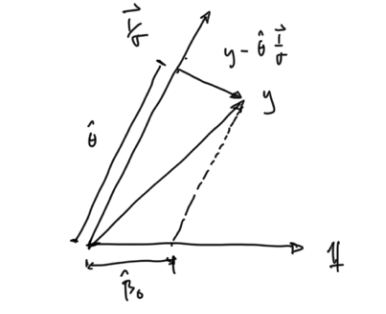
\includegraphics{fig1.png}
  %\caption{Schematic description of the orthogonality of $\hat\beta_0$ and $\hat\theta$ in Egger regression.}
  %\label{fig:1}
%\end{figure}


\begin{theorem}\label{thrm:finite sample}
  Assume
  \begin{align}
    (\y_1,\ldots,\y_n) \mid (\sigma_1^2,\ldots,\sigma_n^2) \sim \N(\theta\mathbbm{1},\diag(\sigma_1^2,\ldots,\sigma_n^2)).
  \end{align}
  %Then  1. the Egger test statistic $\hat\t$ and 2. the Begg test
  % statistic $\hat\tau$ is[[are? but dont want to imply they are joint independent]] conditionally independent of the
  % meta-analysis test statistic $\hat\theta$.
  Then 1. $\hat\t \ind \thetahat \mid \sigma_1,\ldots,\sigma_n$ and 2. $\hat\tau \ind\thetahat \mid \sigma_1,\ldots,\sigma_n$.

  % \begin{enumerate}
  % \item $\hat\t \ind \thetahat \mid \sigma_1,\ldots,\sigma_n$
  % \item $\hat\tau \ind\thetahat \mid \sigma_1,\ldots,\sigma_n$
  % \end{enumerate}
\end{theorem}
\begin{proof}
  \begin{enumerate}
  \item
    % The intercept in Egger's regression is
    % \begin{align}
    %   \hat{\beta}_0 = \frac{1}{n(\m_2-\m_1^2)}\left(\m_2\sum_j\y_j\s_j-\m_1\sum_j\y_j\s_j^2\right) = \sqrt{\frac{RSS}{n-2}}\hat\t.
    %   % \thetahat = \frac{\sum_j\y_j/\sigma_j^2}{\m_2}.
    % \end{align}
    First, for gaussian $\vec\y$, the residual sum of squares in the
    Egger regression, $RSS$, is independent of
    $\hat{\beta}_0$. Second, RSS is also independent of $\hat\theta$
    in light of the remarks preceding the theorem, since
    $\vec{\frac{1}{\sigma}}$ is in the column space of the Egger
    regression. Third,
    $\E(\hat\t \mid \vec\sigma) = \E\left(1/\sqrt{\var(\hat\beta_0)}
      \mid \vec\sigma\right)\E(\hat\beta_0 \mid \vec\sigma)=0$ by OLS
    theory, since the linear model \eqref{model:egger lm} is correct. Therefore,
    \begin{align}
      \cov(\hat\t,\hat\theta \mid \vec\sigma) &= \E(\hat\t \hat\theta \mid \vec\sigma) \\
      % &\left\{\int \middle|\int\right.\\
                                              &= \E\left(\left.\frac{\hat\beta_0\hat\theta}{\sqrt{\var(\hat\beta_0)}} \right| \vec\sigma\right)\\
                                              &=\E\left(\left.\frac{1}{\sqrt{\var(\hat\beta_0)}} \right| \vec\sigma\right)
                                                \E\left(\left.\hat\beta_0\hat\theta \right| \vec\sigma\right)\\
                                              &=\E\left(\left.\frac{1}{\sqrt{\var(\hat\beta_0)}} \right| \vec\sigma\right)
                                                \frac{1}{n(\m_2-\m_1^2)}\frac{1}{\m_2}\E\left(\left.\left(\sum_j \y_j/\sigma_j(\m_2-\m_1/\sigma_j)\right)\sum_j\y_j/\sigma_j^2 \right| \vec\sigma \right),
    \end{align}\comment{vertical bars throughout}
    while the second expectation is
    % \begin{align}
    %   \E\left(\hat\beta_0\hat\theta \mid \vec\sigma\right) &=
    %                                                          \frac{1}{n(\m_2-\m_1^2)}\frac{1}{\m_2}\E\left(\left(\sum_j \y_j\s_j(\m_2-\m_1\s_j)\right)\sum_j\y_j\s_j^2 \mid \vec\sigma \right)\\
    %   &=
    %     \frac{1}{n(\m_2-\m_1^2)}\frac{1}{\m_2}\cov\left(\sum_j \y_j\s_j(\m_2-\m_1\s_j),\sum_j\y_j\s_j^2 \mid \vec\sigma \right)\\
    %                                                        &=\frac{1}{n(\m_2-\m_1^2)}\frac{1}{\m_2} \sum_j\cov(\y_j\s_j(\m_2-\m_1\s_j),\y_j\s_j^2 \mid \vec\sigma)\\
    %   &=\frac{1}{n(\m_2-\m_1^2)}\frac{1}{\m_2} \sum_j\s_j(\m_2-\m_1\s_j)=0.
    % \end{align}
        \begin{align}
             \E\left(\left.\left(\sum_j \y_j/\sigma_j(\m_2-\m_1/\sigma_j)\right)\sum_j\y_j/\sigma_j^2 \right| \vec\sigma \right)
      &=
        \cov\left(\left.\sum_j \y_j/\sigma_j(\m_2-\m_1/\sigma_j),\sum_j\y_j/\sigma_j^2 \right| \vec\sigma \right)\\
                                                           &= \sum_j\cov(\y_j/\sigma_j(\m_2-\m_1/\sigma_j),\y_j/\sigma_j^2 \mid \vec\sigma)\\
      &= \sum_j1/\sigma_j(\m_2-\m_1/\sigma_j)=0.
    \end{align}% [[move preceding fraction to previous display instead of repeating it all these lines. actually should maybe phrase this entire section in terms of sigma since s is not random here, shouldn't be capital S's]].
% [[ideally, show betahat orthog thetahat using geometric/intuitive language before the theorem. theorem can just handle the rss/varbeta part.

  \item As noted in the remarks preceding the theorem statement, $\cov(\vec{\frac{\y}{\sigma}}-\hat\theta \vec{\frac{1}{\sigma}},\vec{\frac{1}{\sigma}})=0$. For any $j$, then, $\cov(\y_j-\hat\theta,\hat\theta \mid \vec\sigma)=\sigma_j^2\cov(\y_j/\sigma_j-\hat\theta/\sigma_j,\hat\theta/\sigma_j \mid \vec\sigma)=0.$ % Given $\vec\sigma$, $\hat\theta$ a projection of $\vec\y$ so $\cov(\y_j-\hat\theta,\hat\theta \mid \vec\sigma)=0$ [[but $\hat\theta$ is just the coefficient of the projection...]].
    Explicitly,
    \begin{align}
      \cov(\y_j-\hat\theta,\hat\theta \mid \vec\sigma) &= \cov(\y_j,\hat\theta \mid \vec\sigma) - \var(\hat\theta \mid \vec\sigma)\\
                                                       &= \cov\left(\left.\y_j, \frac{\y_j/\sigma_j^2}{n\m_2} \right| \vec\sigma\right) - \var\left(\left.\frac{\y_j/\sigma_j^2}{n\m_2} \right| \vec\sigma \right)\\
      &= \frac{1}{n\m_2} - \frac{1}{n\m_2} = 0.
    \end{align}
    Since the data is gaussian,
    $(y_1-\hat\theta,\ldots,y_n-\hat\theta)$ is independent of
    $\hat\theta$ given $\vec\sigma$. Since $\hat\tau$ is a function of
    $(y_1-\hat\theta,\ldots,y_n-\hat\theta)$ given $\vec\sigma$, it
    too is conditionally independent of $\hat\theta$.
  \end{enumerate}
\end{proof}


\begin{corollary}
  Assuming
   \begin{align}
    (\y_1,\ldots,\y_n) \mid (\sigma_1,\ldots,\sigma_n) \sim \N(\theta\mathbbm{1},\diag(\sigma_1^2,\ldots,\sigma_n^2)).
  \end{align}
$\cov(\hat\t,\thetahat)=\cov(\hat\tau,\thetahat)=0.$
\end{corollary}
\begin{proof}
  $\cov(\hat\t,\hat\theta) = \E\cov(\hat\t,\hat\theta\mid\vec\sigma) + \cov\left(\E\left(\hat\t\mid\vec\sigma\right), \E\left(\hat\theta\mid\vec\sigma\right)\right)$. The first term is $0$ by Theorem \ref{thrm:finite sample} and the second since $\E\left(\left.\hat\theta\right|\vec\sigma\right)=\theta$ is constant.
\end{proof}
% theorem. same for begg test. [combine two, same ideas.


% egger finite sample, non-gaussian y. begg case. see notes p1.

In showing that the Egger statistic is independent, normality is only
used to obtain independence of the residual errors from the
coefficient estimate. Writing
\begin{align}
  \cov(\hat\t,\sqrt{n}\hat\theta) =  \cov\left(\hat\t\sqrt{\frac{RSS}{n-2}},\sqrt{n}\hat\theta\right) + \cov\left(\hat\t\left(1-\sqrt{\frac{RSS}{n-2}}\right),\sqrt{n}\hat\theta\right),
\end{align}
the first term is shown to be $0$ in the first part of the proof, and the second is
ordinarily of order $n^{-1/2}$. Therefore, under the general model
\eqref{model:ma}, any correlation between the Egger test statistic and
meta-analysis test statistic vanishes as the number of
studies grows. %  [[whats the point of asy theorem for egger below, then?
% establish asy normality]]
In contrast, without 
the gaussian assumption Begg's test statistic and the meta-analysis test
statistic may be correlated even in the limit, as Theorem \ref{thrm:begg asy}
below shows.



% , i.e., an Egger regression without the intercept term.%, and $1/\vec\sigma$ is in the column space of the egger regression.



\section{Asymptotic, non-parametric study effects}
\label{sec:asy}

We extend the analysis beyond gaussian study effects by considering
the association between the test statistics as the number of studies
$n$
grows. % Besides \eqref{model:ma}, we assume here that the pairs $(\y_1,\sigma_1),(\y_2,\sigma_2),\ldots$ form an iid sequence. Let $\s=1/\sigma$ denote the study precision.


\begin{theorem}\label{thrm:egger asy} Assuming:
  \begin{enumerate}
  \item $(\y_1,\ldots,\y_n) \mid (\sigma_1,\ldots,\sigma_n)$ are independent with
    means $0$ and variances $\sigma_1^2,\ldots,\sigma_n^2$
  \item Existence and
    finiteness of $\mu_1=\lim_{n\to\infty}\m_1=\lim_{n\to\infty}n^{-1}\sum_{j=1}^n 1/\sigma^j$
  \end{enumerate}
  For some  $\delta>0$,
  \begin{enumerate}[resume]
  \item $\sup_j\E\left(\frac{\y_j-\theta}{\sigma_j}\right)^{2+\delta}<\infty$
  \item $\m_2-\m_1^2>\delta$
  % \item $\sum_j\left(\frac{s_j}{j}\right)^{1+\delta}<\infty$
      \item $\sum_j\left(\sigma_j j\right)^{-1-\delta}<\infty$
  \end{enumerate}
  Then
  \begin{align}
    \left.\left(\hat\t,\frac{\hat\theta-\theta}{\sigma_{\hat\theta}}\right) \right| \sigma_1,\ldots,\sigma_n \leadsto \N(0,I).
  \end{align}
\end{theorem}

\begin{proof}
  1. Use the Cramer-Wold device to show
  \begin{align}
    \left(\sqrt{\frac{RSS}{n-1}}\hat\t,\frac{\hat\theta-\theta}{\sigma_{\hat\theta}}\right) \leadsto N(0,I)
    \label{pf:egger asy:cramer}
  \end{align}
  then 2. show $RSS/(n-1)\to_p 1$.

  1. The random variables in the statement, re-written in terms of the study precisions $\s_1,\ldots,\s_n$, are
  \begin{align}
    \hat\t&=\sqrt{\frac{n-1}{RSS}}n^{-1/2}\frac{1}{\sqrt{\m_2(\m_2-\m_1^2)}}\sum_j\y_j\s_j(\m_2-\m_1\s_j)\\
          &=\sqrt{\frac{n-1}{RSS}}n^{-1/2}\frac{1}{\sqrt{\m_2(\m_2-\m_1^2)}}\sum_j(\y_j-\theta)\s_j(\m_2-\m_1\s_j),\\
    \frac{\hat\theta-\theta}{\sigma_{\hat\theta}} &=
                                                    \frac{1}{\sqrt{m_2}}\sum_j(\y_j-\theta)\s_j^2.
  \end{align}

  Given $a,b\in\mathbbm{R}$, the linear combination
  \begin{align}
    a\sqrt{\frac{RSS}{n-1}}\hat\t + b   \frac{\hat\theta-\theta}{\sigma_{\hat\theta}} &=                                                                             n^{-1/2}\sum_{j=1}^n \frac{\s_j^2}{\sqrt{\m_2}}
                                                                                        \left(\frac{a(\m_2/\s_j-\m_1)}{\sqrt{\m_2(\m_2-\m_1^2)}}+b\right)
                                                                                        (\y_j-\theta) 
  \end{align}
  has conditional mean and variance
  \begin{align}
    \E\left(    a\sqrt{\frac{RSS}{n-1}}\hat\t + b   \frac{\hat\theta-\theta}{\sigma_{\hat\theta}}\mid\vec\sigma\right) &= 0\\
    \var\left(    a\sqrt{\frac{RSS}{n-1}}\hat\t + b   \frac{\hat\theta-\theta}{\sigma_{\hat\theta}}\mid\vec\sigma\right) &= a^2+b^2.
  \end{align}
  % [[fix short mid bar]][[add some of the intermediate steps for the variance??]]
  It suffices to show that the linear combination is asymptotically normal, as \eqref{pf:egger asy:cramer} then follows by  the Cramer-Wold device. By the Lyapunov CLT, asymptotic normality follows if for some $\delta>0$, given $\vec\s$,
  \begin{align}
    &\sum_{j=1}^n \E\left|n^{-1/2}\frac{\s_j^2}{\sqrt{\m_2}}
      \left(\frac{a(\m_2/\s_j-\m_1)}{\sqrt{\m_2(\m_2-\m_1^2)}}+b\right)
    (\y_j-\theta) \right|^{2+\delta}\\
    &=\sum_{j=1}^n \left(n^{-1/2}\frac{\s_j}{\sqrt{\m_2}}
      \left(\frac{a(\m_2/\s_j-\m_1)}{\sqrt{\m_2(\m_2-\m_1^2)}}+b\right)\right)^{2+\delta}
    \E\left|\frac{\y_j-\theta}{\sigma_j} \right|^{2+\delta}\\
  \end{align}
  converges to $0$. First, the terms $\E\left|\frac{\y_j-\theta}{\sigma_j} \right|^{2+\delta}$ are assumed bounded. Second, $b\frac{\s_j}{\sqrt{\m_2}}\le b$. Third,
  $$
  \frac{\m_2-\m_2\s_j}{\m_2\sqrt{m_2-\m_1^2}}=\frac{1-\frac{\m_1}{\m_2}\s_j}{\sqrt{\m_2-\m_1^2}}\le\frac{1}{\sqrt{\m_2-\m_1^2}}.
  $$
  Therefore,
  \begin{align}
    \sum_{j=1}^n \left(n^{-1/2}\frac{\s_j}{\sqrt{\m_2}}
    \left(\frac{a(\m_2/\s_j-\m_1)}{\sqrt{\m_2(\m_2-\m_1^2)}}+b\right)\right)^{2+\delta} &\le \sum_{j=1}^n\left(n^{-1/2}\left(b+\frac{1}{\sqrt{\m_2-\m_1^2}}\right)\right)^{2+\delta}\\
                                                                                        &\le \sum_{j=1}^n(n^{-1/2}(b+1/\delta))^{2+\delta}\\
    &= (b+1/\delta)^{2+\delta}n^{-\delta/2}\to 0.
  \end{align}

  2. In terms of the precisions,
  \begin{align}
    \frac{RSS}{n} = \overline{\y^2\s^2}-(\ol{\y\s})^2-\frac{(\ol{\y\s^2}-\m_1\ol{\y\s})^2}{\m_2-\m_1^2}.
  \end{align}
  Let $\mu_k=\lim_{n\to\infty}\frac{1}{n}\sum_{j=1}^n\s_j^k$ for $k=1,2$. Show $\frac{RSS}{n}\to_p 1$ by showing a. $\ol{\y^2\s^2}\to_p 1+\theta^2\mu_2$, b. $\ol{\y\s}\to_p \theta\mu_1$, and c. $\ol{\y\s^2}\to_p \theta\mu_2$. In all 3 cases we use a variant of the LLN (e.g., Chapter 2, Ex. 4.5, of \citet{Rao:73}):  
  % Use [[cite markov lln in rao 1973, or loeve 1950]] in all 3 cases:
  Given independent integrable RVs $X_1,X_2,\ldots,$ and $\delta>0$ such that $\sum_j\E\left|(X_j-\E X_j)/j\right|^{1+\delta < \infty}$, conclude $\left|\frac{1}{n}\sum_{j=1}^nX_j-\frac{1}{n}\sum_{j=1}^n\E X_j\right|\to_{a.s.} 0.$\comment{settle on j or i for default index}
  
  a.
  \begin{align}
    \E\left( (\y_j\s_j)^2 - (1+\theta^2\s_j^2) \right)^{1+\delta}
    &= \E\left( ((\y_j-\theta)\s_j)^2+2\theta(\y_j-\theta)\s_j^2-1 \right)^{1+\delta}\\
    &\le 2^{1+\delta}\left( \E\left(\frac{\y_j-\theta}{\sigma_j}\right)^{2(1+\delta)}+(2\theta\s_j)^{1+\delta}\E\left(\frac{\y_j-\theta}{\sigma_j}\right)^{1+\delta} +1  \right).
  \end{align}
  As $\sup_j\E\left(\frac{\y_j-\theta}{\sigma_j}\right)^{2+\delta}$ is assumed finite for some $\delta>0$, the same holds for $\sup_j\E\left(\frac{\y_j-\theta}{\sigma_j}\right)^{1+\delta}$, and it is assumed that $\sum_j(\s_j/j)^{1+\delta}<\infty$.

  b. With $\delta=2$, $\sum_j\E\left|(y_j\s_j-\theta\mu_1)/j\right|^{1+\delta} = \sum_j \var(\y_j\s_j)=\sum_j1/j^2<\infty$, so $\ol{ys}\to_{a.s.}\theta\mu_1$.
  
  c.
  \begin{align}
    \sum_j\E\left|(\y_j\s_j^2-\theta\s_j^2)/j\right|^{1+\delta}=\sum_j (\s_j/j)^{1+\delta}\E\left|\frac{\y_j-\theta}{\sigma_j}\right|^{1+\delta}<\infty
  \end{align}
  as before.

 
\end{proof}

% When both $\vec\y$ belongs to a scale family, i.e., $(\y_j-\theta)/\sigma_j, j=1,\ldots,n,$  are iid, and the precisions are iid:
Many IID data models meet the conditions of the theorem.

\begin{corollary}
  Assuming: 1. $(\y_1,\ldots,\y_n) \mid (\sigma_1,\ldots,\sigma_n)$ are
  independent with means $0$ and variances
  $\sigma_1^2,\ldots,\sigma_n^2$.
  2. $((\y_1-\theta)/\sigma_1,\ldots,(\y_n-\theta)/\sigma_n) \mid
  (\sigma_1,\ldots,\sigma_n)$ follow a common distribution such that
  for some $\delta>0$,
  $\E((\y-\theta)/\sigma\mid\sigma)^{2+\delta}<\infty$. 3. The precisions
  $\s_1,\s_2,\ldots$ are IID, non-constant, with a finite second
  moment. % For some $\delta>0$,
  % $\sup_j\E\left(\frac{\y_j-\theta}{\sigma_j}\right)^{2+\delta}<\infty$,
  % $\m_2-\m_1^2>\delta$,
  % $\sum_j\left(\frac{\s_j}{j}\right)^{1+\delta}<\infty$. Existence and
  % finiteness of
  % $\mu_1=\lim_{n\to\infty}\m_1=\lim_{n\to\infty}n^{-1}\sum_{j=1}^n
  % 1/\sigma^j$. 
  Then almost surely,
  \begin{align}
    \left.\left(\hat\t,\frac{\hat\theta-\theta}{\sigma_{\hat\theta}}\right)\right| \sigma_1,\sigma_2,\ldots,\sigma_n \leadsto N(0,I).
  \end{align}
\end{corollary}

\begin{proof}
  $\m_2-\m_1^2\to \var(\s)$ almost surely, with $0<\var(\s)<\infty$, so almost surely there is a random $\delta>0$ such that $\m_2-\m_1^2>\delta$. By a truncation argument (e.g., Ex. 2.3.25 of \citet{dembo:16}) the assumed moment condition on $\s$ likewise implies $\sum_j (\s_j/j)^{1+\delta}$ converges almost surely for any $1<\delta\le 2$.
  % [[maybe can prove under the assumption that $S$ has a $2+\delta$ moment using dembo notes thrm 2.3.17 (but need to de-mean s). but seems don't need this assumption, can use dembo notes 2.3.25(a).]]
  % Taking $\delta=1$,
  % \begin{align}
  %   \sum_j\left(\frac{\s_j}{j}\right)^{1+\delta} \le \sqrt{\sum_j\s_j^2\sum_j1/j^2} \le \sqrt{\frac{1}{\sum_j\s_j^2} \
  % \end{align}
\end{proof}

% old non-conditional version of asy egger theorem. assumes S_j are iid also.
% \begin{theorem} Under \eqref{model:ma}, Assuming $ES^4<\infty$.
%   \begin{align}
%     \begin{pmatrix} t \\ (\thetahat-\theta)/\sigma_{\hat\theta} \end{pmatrix}
%     \leadsto \mathcal{N}(0,I).
%     % \mathcal{N}\left(0,\begin{pmatrix}
%     %     1 & 0\\
%     %     0 & 1
%     %   \end{pmatrix}
%     % \right)      
%   \end{align}
% \end{theorem}

% \begin{proof}

%   1. formula for $\hat\t=\frac{\hat\beta_0}{\sqrt{\hat\var\hat\beta_0}}$:
%   \begin{align}
%     \hat\t = \sqrt{\frac{n-1}{RSS}}n^{-1/2}\frac{1}{\sqrt{\m_2(\m_2-\m_1^2)}}
%     \sum_j\y_j\s_j(\m_2-\m_1\s_j).
%   \end{align}

%   2. simplify formula in terms of an iid sum centered with unit variance:
%   \begin{align}
%     \hat\t = n^{-1/2}\frac{1}{\sqrt{\mu_2(\mu_2-\mu_1^2)}}
%     \sum_j(\y_j-\theta)\s_j(\mu_2-\mu_1\s_j) + o_P(1)
%   \end{align}

%   a. Since the regression of $\vec{\frac{\y}{\sigma}}$ on $\vec{\frac{1}{\sigma}}$ is correctly specified, $RSS/(n-2)\to_p \var(\y/\sigma_j\mid \sigma_j)=1$.

%   b.
%   \begin{align}
%     &n^{-1/2}\sum_j\y_j\s_j(\m_2-\m_1\s_j) - n^{-1/2}\sum_j(\y_j-\theta)\s_j(\mu_2-\mu_1\s_j)\\
%     &=    n^{-1/2}\sum_j(\y_j-\theta)\s_j(\m_2-\m_1\s_j) - n^{-1/2}\sum_j(\y_j-\theta)\s_j(\mu_2-\mu_1\s_j)\\
%     &=    n^{-1/2}\sum_j(\y_j-\theta)\s_j(\m_2-\mu_2) - n^{-1/2}\sum_j(\y_j-\theta)\s_j^2(\m_1-\mu_1)\\
%     &=O_p(1)o_p(1)-O_p(1)o_p(1)\\
%   \end{align}
%   assuming $\E\s^2<\infty$ [[clt appeal in last equality with $\s_j^2$ means we need $E(\s^4)<\infty$.

%   3. asymptotic normality of $\hat\theta$
%   \begin{align}
%     \sqrt{n}\begin{pmatrix}
%       n^{-1}\sum_j\y_j\s_j^2-\theta\mu_2\\
%       n^{-1}\sum_j\s_j^2-\mu_2
%     \end{pmatrix}
%     \leadsto \mathcal{N}\left(0,
%     \begin{pmatrix}
%     \mu_2+\theta^2(\mu_4-\mu_2^2) & \theta(\mu_4-\mu_2^2)\\
%                                   & \mu_4-\mu_2^2
%                                 \end{pmatrix}
% \right).
%   \end{align}
%   [[so again, need 4th moments of s]]
%   Apply delta method with $(x,y)\mapsto x/y$ to get
%   \begin{align}
%     \sqrt{n}(\hat\theta-\theta)\mu_2 \leadsto \mathcal{N}(0,1).
%   \end{align}

%   4.
%   \begin{align}
%     \cov\left(\sqrt{\frac{RSS}{n-2}}\hat\t,\sqrt{n}\hat\theta\right) &=
%                                                             \E\left( \cov\left(\frac{\sum_j\z_j(\m_2-\m_1\s_j)}{\sqrt{\m_2(\m_2-\m_1^2)}},\frac{\frac{1}{n}\sum_j\z_j\s_j}{\m_2} \mid\vec\sigma\right)\right)\\
%                                                           &=\E\left(\frac{1}{\m_2}\frac{1}{\sqrt{\m_2(\m_2-\m_1^2)}}\frac{1}{n}\sum_j\cov\left(\z_j(\m_2-\m_1\s_j),\z_j\s_j \mid \vec\sigma\right)\right)\\
%                                                           &=\E\left(\frac{1}{\m_2}\frac{1}{\sqrt{\m_2(\m_2-\m_1^2)}}\frac{1}{n}\sum_j\s_j(\m_2-\m_1\s_j) \right)=0.\\
%   \end{align}
%   Since $\sqrt{\frac{RSS}{n-2}} \to_p 1$, $\cov(\hat\t,\sqrt{n}\hat\theta)\to 0$.[[integration to the limit here?]]

%   5. Putting parts together,
%   \begin{align}
%     &\sqrt{n}\begin{pmatrix}
%       \hat\t/\sqrt{n}\\ n^{-1}\sum_j\y_j\s_j^2-\theta\mu_2\\ n^{-1}\sum_j\s_j^2-\mu_2 
%     \end{pmatrix} \\
%     &= o_p(1) +
%     \begin{pmatrix}
%       \frac{n^{-1/2}}{\sqrt{\mu_2(\mu_2-\mu_1)^2}}\sum_j(\y_j-\theta)\s_j(\mu_2-\mu_1\s_j)\\
%       \sqrt{n}(n^{-1}\sum_j\y_j\s_j^2-\theta\mu_2)\\
%       \sqrt{n}(n^{-1}\sum_j^2-\mu_2)
%     \end{pmatrix} \leadsto \mathcal{N}\left(0,
%     \begin{pmatrix}
%       1 & 0 & 0\\
%       & \mu_2+\theta^2(\mu_4-\mu_2^2) & \theta(\mu_4-\mu_2^2)\\
%       & & \mu_4-\mu_2^2
%     \end{pmatrix}\right).
%   \end{align}
%   Then the delta method gives the conclusion of the theorem.
% \end{proof}

% [[define moments mu somewhere]]
% mention begg test vairance bias. begg reduction to get rid of sigmatheta. cite other michael paper, put
% proof there. scale family assumption.

The corresponding analysis for Begg's statistic is relatively complicated due to the statistics 
% $\hat\theta$.% : scale family with with basic pdf $f_\z$,
% % $\E(\z)=0,\var(\z)=1$, etc.
% Analysis is complicated by terms
$\sigma_{\hat\theta}$ and $\hat\theta$ common to the terms of the
double sum \eqref{defn:kendalls tau}. We impose several simplifying assumptions. % additional assumptions to
% obtain asymptotic normality of begg's statistic $\hat\tau$ and the
% meta-analysis test statistic
 First, as noted in Section \ref{sec:background:location invariance},
$\hat\tau$ is invariant to shifting the location of the study effects,
$\vec\y\mapsto\vec\y+\theta$, so there is no loss in assuming
$\theta=0$:
\begin{align}
  \E(\y_1,\ldots,\y_n \mid \sigma_1,\ldots,\sigma_n) = 0.
  \label{assumption:begg mean 0}
\end{align}
Second, the $O(1/n)$ terms $\sigma_{\hat\theta}$ are asymptotically negligible
in many common situations \citep{michael:inpress-a},
\begin{align}
  \hat\tau &= {n\choose 2}^{-1}\sum_{j<k}2\left\{\left(\frac{\y_j-\hat\theta}{\sigma_j}-\frac{\y_k-\hat\theta}{\sigma_k}\right)(\sigma_j-\sigma_k)>0\right\}-1 + o_P(n^{-1/2}).
  % &=  {n\choose 2}^{-1}\sum_{j<k}2\left\{\frac{\z_j-\z_k}{\s_j-\s_k}<\hat\theta\right\}-1 + o_P(n^{-1/2}).
      \label{eqn:begg no sigma_theta}
\end{align}
Next, let $\z_j=\y_j/\sigma_j,j=1,\ldots,n,$ denote the standardized effect
sizes. From \eqref{model:ma}, $\var(\z)=1$ and by \eqref{assumption:begg mean 0}, $\E(\z)=0$. We further assume that 
$\z_1,\ldots,\z_n,$ follow a common distribution, i.e., the study
effects $\y_1,\ldots,\y_n,$ belong to a scale family. Finally, we assume the study precisions $(\s_1,\ldots,\s_n)$ are IID. % [[We consider the marginal behavior of $(\hat\tau,\hat\theta)$ marginally over the study variances, rather than the conditional analyses prevoiusly considered.]] 
In summary,
\begin{align}
    \label{model:scale}
  \begin{split}
    \z_1,\ldots,\z_n &\overset{IID}{\sim} F_Z\\
    \s_1,\ldots,\s_n &\overset{IID}{\sim}  F_S\\
    % \z_j &\sim -\z_j,\\
    \z_j \mid \s_j &\sim \z_j,\\
    \y_j&=\z_j/\s_j,j=1,\ldots,n.
  \end{split}
\end{align}
Rewritten in
terms of the standardized effect sizes and their precisions, \eqref{eqn:begg no sigma_theta} is
\begin{align}
  \hat\tau &=  {n\choose 2}^{-1}\sum_{j<k}2\left\{\frac{\z_j-\z_k}{\s_j-\s_k}<\hat\theta\right\}-1 + o_P(n^{-1/2}).
             \label{eqn:begg simplified}
\end{align}

The double sum may be viewed as a U-statistic with estimated parameter
$\hat\theta$ \citep{nolan:88}. The estimate is ordinarily of order
$1/\sqrt{n}$ and affects the asymptotics, and Begg's test,
ignoring this effect, can be biased \citep{michael:inpress-a}. The
following result includes the correct asymptotic distribution under
the IID model \eqref{model:scale}.

\begin{theorem}\label{thrm:begg asy} Assuming:
  \begin{enumerate}
    \item the IID model \eqref{model:scale}
    \item $0 < \E \s^2 < \infty$
    \item $\int_{-\infty}^\infty f_\z(z)^2 dz < \infty$
      \comment{add any other assumptions after drafting inpress-b}
  \end{enumerate}
  Then
  \begin{align}
    &\begin{pmatrix} \sqrt{n}\hat\tau \\ (\thetahat-\theta)/\sigma_{\hat\theta} \end{pmatrix} 
    % \leadsto\\
    % &\mathcal{N}\left(0,\begin{pmatrix}
    %     \frac{4}{9}+\frac{4\left(\E|\s-\s'|\right)^2}{\E\s^2}\E(f_\z(\z))\left(\E(f_\z(\z))-2\E(\z F_\z(\z))\right) &
    %        \frac{2\E|\s-\s'|}{\E\s^2}\left(\E f_\z(\z)-\E(\z F_\z(\z))\right)\\
    %      & 1/\mu_2
    %   \end{pmatrix}
    % \right)      .
  \end{align}
  is asymptotically normal with
  \begin{align}
    \var(\sqrt{n}\hat\tau) &\to \frac{4}{9}+\frac{4\left(\E|\s-\s'|\right)^2}{\E\s^2}\E(f_\z(\z))\left(\E(f_\z(\z))-2\E(\z F_\z(\z))\right),\\
    \cov(\sqrt{n}\hat\tau,(\thetahat-\theta)/\sigma_{\hat\theta} ) &\to           \frac{2\E|\s-\s'|}{\sqrt{\E\s^2}}\left(\E f_\z(\z)-\E(\z F_\z(\z))\right),\\
    \var((\thetahat-\theta)/\sigma_{\hat\theta} ) &\to 1.
  \end{align}
\end{theorem}
The theorem follows from a lemma given in \citet{michael:inpress-b} that, drawing on
the theory of U-processes \citep{nolan:88}, rewrites \eqref{eqn:begg simplified} as an asymptotically equivalent IID sum to which the CLT may
be applied. Let
\begin{align}
  % &\hat\tau(\theta) = ...\\
  % &\tau:\theta \to \E(\hat\tau(\theta))\\
  \Pi\hat\tau(\theta):\theta\mapsto
  2\left(\frac{1}{n}\sum_{j=1}^n2\P\left(\frac{\z_j-\z}{\s_j-\s}<\theta \mid \z_j,\s_j\right)-1\right) - \left(2\P\left(\frac{\z-\z'}{\s-\s'}<\theta\right)-1\right).
\end{align}
\begin{lemma} Under the assumptions of Theorem \ref{thrm:begg asy},
  \begin{align}
    \sqrt{n}\hat\tau = \sqrt{n}\left(\hat\theta 2\E(f_\z(\z))\E|\s-\s'| + \Pi\hat\tau(0) \right) + o_P(1)
  \end{align}
\end{lemma}

% \begin{proof}[of theorem [[begg]]]
% Conditionally on $\vec\sigma$, equivalently, on $\vec\s$, the Lemma gives an iid sum asymptotically equivalent to $\hat\tau$. The same holds for the meta-analysis statistic $\hat\theta$. The CLT therefore applies.[[maybe give variance calculations.]]
% \end{proof}

% [[is term always ge 0?]]

The asymptotic covariance between $\hat\tau$ and $\hat\theta$ given in
Theorem \ref{thrm:begg asy} depends on both the distribution of the
study precisions, through the parameter
\begin{align}\label{defn:begg variance bias}
  \frac{\E|\s-\s'|}{\sqrt{\E\s^2}},
\end{align}
and that of the study effects, through the parameter
\begin{align}\label{defn:begg effect bias}
  \zdiff(F_\z) = \E f_\z(\z)-\E(\z F_\z(\z)).
\end{align}
The ratio \eqref{defn:begg variance bias} approaches $0$ as the
precision distribution approximates a nonzero constant. A loose upper
bound of $\sqrt{2}$ follows from
$(\E|\s-\s'|)^2 \le \E((\s-\s')^2) = 2\var(\s) \le 2\E(\s^2)$.
\citet{michael:inpress-a} gives a tight upper bound of $\sqrt{2/3}$.
 
The parameter $\zdiff(F_\z)$ takes a larger range of values and also
determines the sign of the correlation, in turn determining whether
the power of the subsequently conducted meta-analysis will be too low
or too high. For some distributions of $\z$, $\zdiff$ is $0$. For
example, for standard normal $\z$,
$\E f_\z(\z)=\E(\z F_\z(\z))=1/(2\sqrt{\pi})$, and for centered and
scaled uniform $\z$, $\E f_\z(\z)=\E(\z F_\z(\z))=1/(2\sqrt{3})$. When
the standardized effects follow these distributions, Begg's test does
not bias the meta-analysis, under the conditions of Theorem
\ref{thrm:begg asy}.

In general, however, $\zdiff$ may be arbitrarily
large. In terms of the centered but not necessarily scaled study effects $\y=\sigma\z$,
\begin{align}
  \int f_\z(z)^2 = \sigma\int f_\y(y)^2.
\end{align}
The expression on the right may blow up due to either factor $\sigma$
or $f_\y(y)^2$. An example of the former is Student's t. As the
degrees of freedom $p$ approach $2$ from above, $\sigma\to\infty$,
while $\int f_\y^2(y)\propto \int (1+y^2/p)^{1+p}$ is bounded away
from $0$. An example of the latter is any unbounded density that
diverges faster than $1/\sqrt{x}$, such as the ``peaked''
distribution,
% $$
% f_\z(z)\propto |z|^p, p>-1, 0< |z| < c,
% $$
\begin{align}
f_\y(y)=|y|^p \text{ on }|y|<\left(\frac{p+1}{2}\right)^{\frac{1}{p+1}}, \hspace{10px}p>-1. 
\label{defn:peaked pdf}
\end{align}
For this density, $\int f^2_\y(y) \propto \int |y|^{2p}\to\infty$ as
$p \downarrow -1/2$, while  for $p=-1/2$,
$\sigma^2=\int y^2 f_\y(y)=1/5(1/4)^4$.\comment{check} Another example is a centered, symmetric beta distribution with common shape parameter $p$,
\begin{align}
  f_\y(y)=\frac{\left(1/4-y^2\right)^{p-1}}{\B(p,p)}\text{ on }|y|<1/2, p>0.
  \label{defn:centered beta}
\end{align}
Here $\int f_\y^2(y) \propto (1/4-y^2)^{2(p-1)} \to \infty$ as
$p \downarrow 1/2$. While the density \eqref{defn:peaked
  pdf} is increasingly peaked as $\int f_\y^2(y)\to\infty$, with mass
moving to the origin, the centered beta \eqref{defn:centered beta} is
increasingly U-shaped, with mass moving to $\pm 1/2$.

Though $\zdiff\to\infty$ due either to $\sigma\to\infty$ or
$\E f_\y=\int f_\y^2(y)\to\infty$, the two possibilities say different things
about the operational characteristics of the publication bias
tests. When $\sigma$ is large, the basic meta-analysis model
\eqref{model:ma} is nearly violated and there are other difficulties
with attempting a meta-analysis. For example, the fixed effects
estimator $\hat\theta$ may have a poor rate of convergence under the
CLT. A large value of $\E f_Z=\int f_\z^2$ poses problems specifically
for Begg's test. Student's t and the densities \eqref{defn:peaked
  pdf}, \eqref{defn:centered beta}, are examined using synthetic data in Section
\ref{sec:simulation}.

% [[for constant c]].
% After scaling $\z$ to have unit variance per model \eqref{model:scale}, for $p>-1/2$,
% \begin{align}
%   \E(f_\z(\z)) &=  \frac{(p+1)^{5/2}}{2 \sqrt{p+3} (2 p+1)} \to \infty\text{ as } p\to -1/2
%   % \\\E(\z F_\z(\z)) &= 2^{\frac{1}{p+1}-\frac{1}{2}} (p+1)^{-\frac{p+2}{p+1}} \sqrt{\frac{\left(2^{-\frac{1}{p+1}}
%   %                   (p+1)^{\frac{1}{p+1}}\right)^{p+3}}{p+3}} (p+3) \left(\frac{\left(2^{-\frac{1}{p+1}}
%   %                     (p+1)^{\frac{1}{p+1}}\right)^{p+1}}{(p+2) (2 p+3)}+\frac{p+1}{2 p+4}\right)                \\
%   \\\E(\z F_\z(\z)) &= \frac{\sqrt{u^{p+1}(p+3)}}{\sqrt{2}(p+1)^{p+2}} \left(\frac{u^{p+1}}{(p+2) (2 p+3)}+\frac{p+1}{2 p+4}\right)               \to \sqrt{5}/8\text{ as }p\to -1/2,\\
%                       \text{with }u&=2^{-\frac{1}{p+1}}
%                     (p+1)^{\frac{1}{p+1}}.[[check limit]]
% \end{align}
% Therefore $\zdiff \to \infty$ as $p\downarrow -1/2$, as the peakedness at 0 of
% $f_\z$ increases.

When $\zdiff$ is large, screening out data for which Begg's test does
not give a significant result then affects in kind the positively
correlated meta-analysis test statistic, reducing its power. % [[Loss of power seems to be the main consequence of this bias:]]
Very negative $\zdiff$, which would lead to poor FPR control on the meta-analysis, does not appear to be as significant an issue.
\begin{theorem}\label{thrm:extremization} Let $A$ denote the set of
  monotonic differentiable real-valued functions such that
  $\lim_{z\to -\infty}F(z)=0,\lim_{z\to \infty}F(z)=1,\int z F'=0,
  \int z^2 F'=1.$ Let lower-case $f$ denote the derivative $F'$ for $F\in A$.
  \begin{enumerate}
  \item The functional $F \mapsto \int (F'(z))^2 dz=\int f(z)^2$ is
    convex on the set of differentiable functions with
    square-integrable derivatives, and is minimized on $A$ by
    $f(z) \propto 0\vee (1-z^2)$, with value $3/(5\sqrt{5})$.
  \item The functional
    $F \mapsto \int z F(z) F'(z)dz = \int z F(z) f(z)dz$ is concave on $A$ and is maximized when $f$ is a centered and scaled uniform
    distribution, with value $1/(2\sqrt{3})$.
  \item The functional $F \mapsto \int (F'(z))^2 dz -  \int z F(z) F'(z)dz=\zdiff(F)$ is convex and is minimized on $A$ by $f(z)$ of the form $0\vee a\cosh(z/\sqrt{2})+b, a,b\in\mathbb{R}.$
  \end{enumerate}
\end{theorem}
\begin{proof}
  \begin{enumerate}
  \item For $\lambda\in [0,1]$,
    \begin{align}
      \lambda \int f^2 + (1-\lambda)\int g^2 - \int (\lambda f + (1-\lambda)g)^2 = \lambda(1-\lambda)\int (f-g)^2 \ge 0 .
    \end{align}
    
    For the minimization, see, e.g., Chapter 14, Ex. 8, of \citet{vandervaart:00}.
  \item For $\lambda\in [0,1]$, $F,G\in A$,
    \begin{align}
      &\int z(\lambda F + (1-\lambda)G)(\lambda f+ (1-\lambda) g) - \lambda\int z F f - (1-\lambda)\int z G g\\
      &=-\lambda(1-\lambda)\int z(f-g)(F-G)\\
      &= -\lambda(1-\lambda)\left(\left.\frac{z}{2}(F-G)^2 \right|_{-\infty}^\infty - \frac{1}{2}\int(F-G)^2\right)\\
      &= \frac{1}{2}\lambda(1-\lambda)\int(F-G)^2\ge 0.
    \end{align}
    
    For the maximization,
    \begin{align}
      \int_{-\infty}^{\infty}zF(z)f(z) =
      \int_{-\infty}^{\infty}z\left(F(z)-\frac12\right)f(z)
      \le \left(\int_{-\infty}^\infty\left(F(z)-\frac12\right)^2 f(z)\right)^{\frac12} = \frac{1}{2\sqrt{3}},
    \end{align}
    and this bound is achieved by a centered and scaled uniform, $f_\z(z)=\{-1/2\le \sigma z \le 1/2\}\sigma, \sigma=1/(2\sqrt{3}).$%$f_\z(z)=\{-1/2\le 2\sqrt{3}z \le 1/2\}2\sqrt{3}.$
    % [[assuming $z(F-G)^2\to 0$...follows from moment assumptions on A]]

    % The variational calculus gives conditions for
    % stationarity of $\int z F F'$ subject to
    % $\int F'=1, \int z F'=0, \int z^2 F'=1$. The Lagrangian is
    % $
    % z F F' - \lambda_1 z F'-\lambda_2z^2 F'
    % $
    % with Euler-Lagrange equation $F=\lambda_1+2\lambda_2 3$, implying
    % a density $f$ proportional to a constant.

  \item Convexity follows from the previous parts since the sum of convex functions is convex.

    The variational calculus gives a stationary point for $F\mapsto\zdiff(F)$ subject to $\int z f(z)=0,\int f(z)=\int z^2 f(z)=1$. The % lagrangian is $(F')^2-zFF'-\lambda_1zF'-\lambda_2z^2F'$
    Euler-Lagrange equation is $2F''-F=\lambda_1+\lambda_2z$, with general solution of the form
    \begin{align}
      F(z)&=a_1e^{z/\sqrt{2}}+a_2e^{-z/\sqrt{2}}+\lambda_1+\lambda_2z\\
      f(z)&=(a_1e^{z/\sqrt{2}}-a_2e^{-z/\sqrt{2}})/\sqrt{2}+\lambda_2, \qquad a_1,a_2,\lambda_1,\lambda_2\in\mathbb{R}.
    \end{align}
    The objective $\zdiff$ is unchanged under
    $F(\cdot)\mapsto 1-F(-\cdot)$, i.e., negating the random variable
    $\z$. Since $\zdiff$ is convex, any minimal value must then occur at the
    distribution of a symmetric random variable, implying that
    $a_1=a_2$ and the density has the form
    \begin{align}
      f(z)&= a \cosh(z/\sqrt{2})+b,\qquad a,b\in\mathbb{R}.
    \end{align}    
  \end{enumerate}
\end{proof}
% While Theorem \ref{theorem:extremization} deExact minimization of $\zdiff$, but
The first two parts of Theorem \ref{thrm:extremization} imply a lower bound
\begin{align}
\zdiff \ge 3/(5\sqrt{5})-1/(2\sqrt{3})\approx -0.02.\label{eqn:zdiff lb}
\end{align}
The values $a,b,$ of the minimizer
$0\vee a\cosh(z/\sqrt{2})+b$ in the third part do not appear to have
a closed form. Numerical methods give densities of this form for which
$\zdiff\le -0.19$, so the bound \eqref{eqn:zdiff lb} is at worst loose by the
hundredths place.
% This bound is not achieved by the uniform distribution given in the Theorem. As mentioned earlier, $\zdiff=0$ for the centered and scaled uniform.\comment{ maybe mention difficulty with finding cosh minimum]]}

% begg test.

% give asy joint distribution of test stat and theta.fe.
% asy covariance depends on z and s. whether 0 or not depends on z. s
% distribution can grow or diminish it. 0 for gaussian z, unif z. examples of power law, wehre it isn't 0. give depenendence for power law.


% egger test 

\section{Simulation}\label{sec:simulation}

We use synthetic data to investigate the effect on a meta-analysis of
conditioning the data on a non-significant publication bias test
outcome. First, a synthetic body of studies
$(\y_1,\sigma_1,\ldots,\y_n,\sigma_n)$ is generated under model
\eqref{model:ma}. Next, Egger's test for publication bias,
$$
|\hat\t|>t_{n-2,1-\alpha_0/2}
$$ and Begg's test for publication bias
$$
\sqrt{9n/4}|\hat\tau| > \Phi^{-1}(1-\alpha_0/2)
$$
are carried out at significance level $\alpha_{0}$. Finally, the test
for a non-zero grand mean in the meta-analysis,
$$
\hat\theta/\sigma_{\hat\theta} > \Phi^{-1}(1-\alpha_1/2)
$$
is carried out at significance level $\alpha_1$. The process is
iterated $10,000$ times, giving a set of $10,000$\comment{finalize these reps} triples of rejection
indicators. With these we approximate the error rates of the
meta-analysis test conditional on not rejecting during the publication bias
test.

\subsection{Parameters of simulation}
In generating the body of studies
$(\y_1,\sigma_1,\ldots,\y_n,\sigma_n)$ we considered three families for
the distribution of the responses $\vec\y$:
\begin{enumerate}
\item Student's t distributions with degrees of freedom ranging
  between $(2,6)$. When the degrees of freedom are large, the data
  approaches the gaussian model, in which Theorem \ref{thrm:finite
    sample} asserts the publication bias tests exert no influence on the
  meta-analysis distribution. When the degrees of freedom approach $2$, the
  variance blows up and the data approach the boundary of the basic meta-analysis model
  \eqref{model:ma}.
\item The power law-type distribution \eqref{defn:peaked pdf}, with the exponent $p$
  in the range $(-1,0]$. When the exponent is $p=0$, the distribution is a centered
  and scaled uniform, for which $\zdiff=0$, with the peakedness about the origin increasing as $p\to -1$. When $p\to -1/2$,
  $\zdiff\to\infty$, posing difficulties for Begg's test according to
  Theorem \ref{thrm:begg asy}. For $1<p\le.5$, the theorem is
  inapplicable as $\E f_\z$ is not finite, and only perhaps
  suggestive of the behavior of Begg's test.
\item Symmetric and centered beta distributions \eqref{defn:centered beta}, with common shape
  parameter $p$ in the range $[.1,1]$. When $p=1$, the distribution is
  again a centered and scaled uniform. When $p\to 0$, the density
  becomes increasingly U-shaped. For $p<1/2$ Theorem \ref{thrm:begg
    asy} is again only suggestive as $\E f_\z$ is not finite.
\end{enumerate}
In all cases, the distribution of the standard deviations was uniform
on $[1,4]$, following \citet{lin:18}. The meta-analysis sample size
was $n=25$ or $n=75$, following \citet{begg:94a}, who based the choice
on literature reviews of the medical and social sciences literature,
respectively. The grand mean $\theta$ was $0$ or $.2$, with $0$
representing the null case in the meta-analysis test. The significance
level of the screening publication bias test $\alpha_0$ was
$0.05$ or $0.15$ following recommendations in \citet{egger:97}, \cite{begg:94b}, and elsewhere\comment{check}, while in all cases
the level of the meta-analysis test was $\alpha_1=.05$, a standard recommendation
\citep{konstantopoulos:19}. \comment{[[parameters may be adjusted, cite
github.]]}\comment{finalize parameters}

\subsection{Results of simulation}
Main results are given in Tables \ref{table:power 0} and \ref{table:power 0.2}.
\begin{enumerate}
\item Student's t distributions. The power of the meta-analysis is
  similar whether a publication bias test is used or not.  That power
  is around the nominal rate when the degrees are in the range
  $4\text{--}6$ or larger, dropping as the degrees of freedom approach $2$. The
  drop is expected as model \eqref{model:ma} does not hold for degrees
  of freedom $\le 2$. It is unrelated to screening and attributable to
  the slow CLT convergence of of averages such as 
  $\hat\theta$ under these distributions.

\item Power law-type distributions. The power of Begg's test drops as
  the peakedness increases, while Egger's test is consistent. % The
  % drop is greater for the larger sample size, as discussed further below.
  The behavior is
  expected from Theorem \ref{thrm:begg asy}, which shows the
  dependence of $\cov(\hat\tau,\hat\theta)$ on $\E f_\z$, and Theorem
  \ref{thrm:egger asy}, which asserts that $\hat\t$ and $\hat\theta$
  are asymptotically independent.

\item Beta distributions. As with the power law-type distribution, the
  power of Begg's test drops relative to Egger's test as the
  distribution becomes less uniform and increasingly U-shaped. This
  result, too, is expected from Theorem \ref{thrm:begg asy}, as the
  change in shape corresponds to increasing $\E f_\z$.  
\end{enumerate}
% in figs, have xaxis consist of both the distribution parameter and z diff?

In the problem area, i.e., Begg's test for very peaked or very
U-shaped distributions, Tables \ref{table:power 0} and
\ref{table:power 0.2} reveal two other contributors to lower
power. The first is that the power is poorer as the sample size
increases. For example, for the most peaked power law-type
distribution in Table \ref{table:power 0}, the power of Begg's test
drops from a reasonable $.045$ when $n=25$ to $.007$ when $n=75$. In
contrast, for Student's t, the power improves with sample size, as the
CLT approximation improves. Theorem \ref{thrm:begg asy} is qualitative
in that it provides no rates of convergence to the asymptotic
covariance between $\hat\tau$ and $\hat\theta$. Evidently the
asymptotic covariance overstates the severity, particularly for the
relatively small values of $n$ typical of meta-analyses. A more
refined asymptotic analysis might offer a more accurate picture of the
finite sample behavior.

A second, less dramatic contributor to lower power is a larger nominal level for
the screening publication bias test $\alpha_0$. \comment{For example, [[]]} This
effect is at odds with the frequent recommendation to opt for
higher nominal levels in testing for publication bias as a way to
boost power \citep{begg:94b,egger:97,macaskill:01}. The
magnitude of a test statistic being inversely related to the p-value, 
the magnitude of the publication bias test statistic conditional on being
$\ge \alpha_0$ tends to be smaller as $\alpha_0$ is
larger. Consequently the positively correlated meta-analysis test
statistic also tends to be smaller in magnitude, reducing the power
of the meta-analysis test. See Fig. \ref{fig:alpha_0}.
% \begin{figure}
%   \begin{minipage}{.5\textwidth}
%     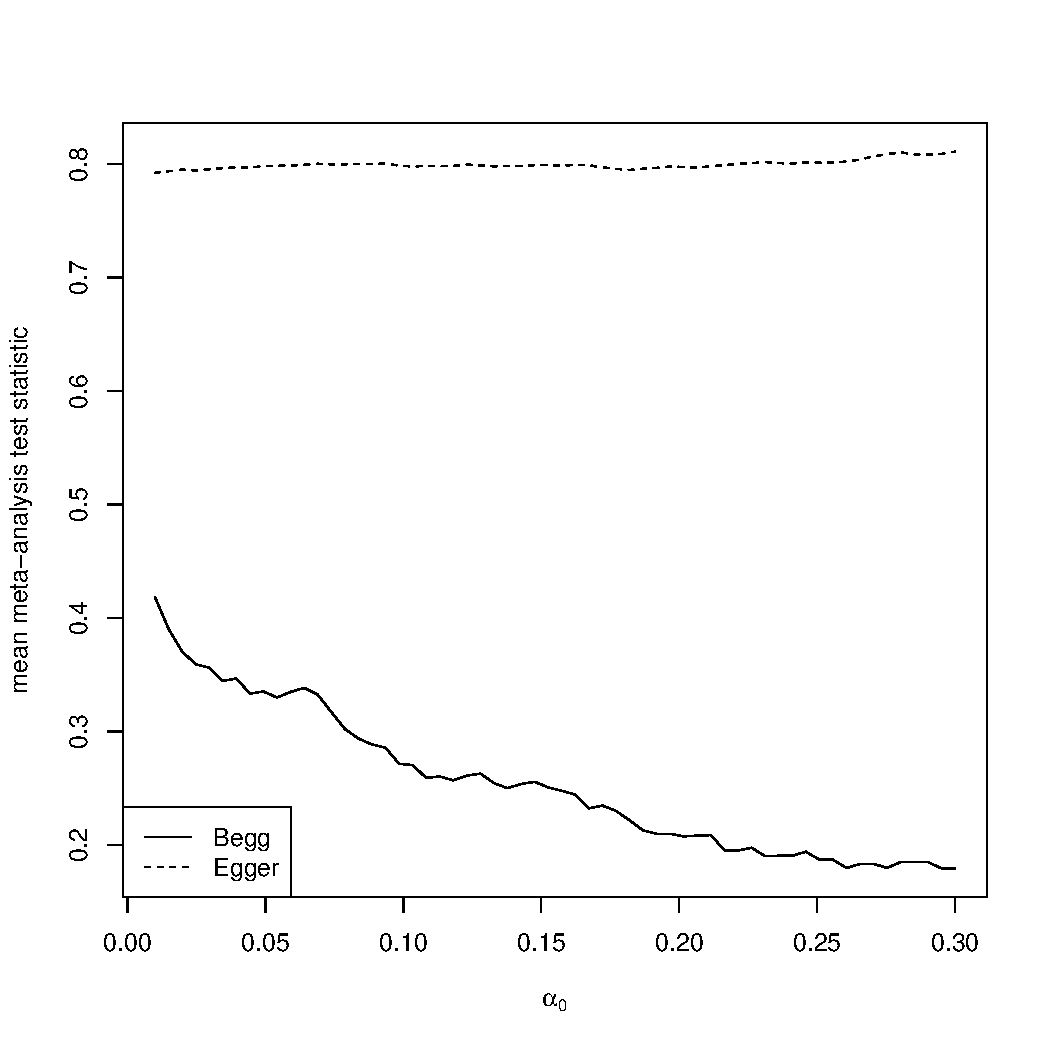
\includegraphics[width=\linewidth]{fig_alpha_0_power.pdf}
%     \caption{Power-type $f_\z$.}
%   \end{minipage}
%   \begin{minipage}{.5\textwidth}
%     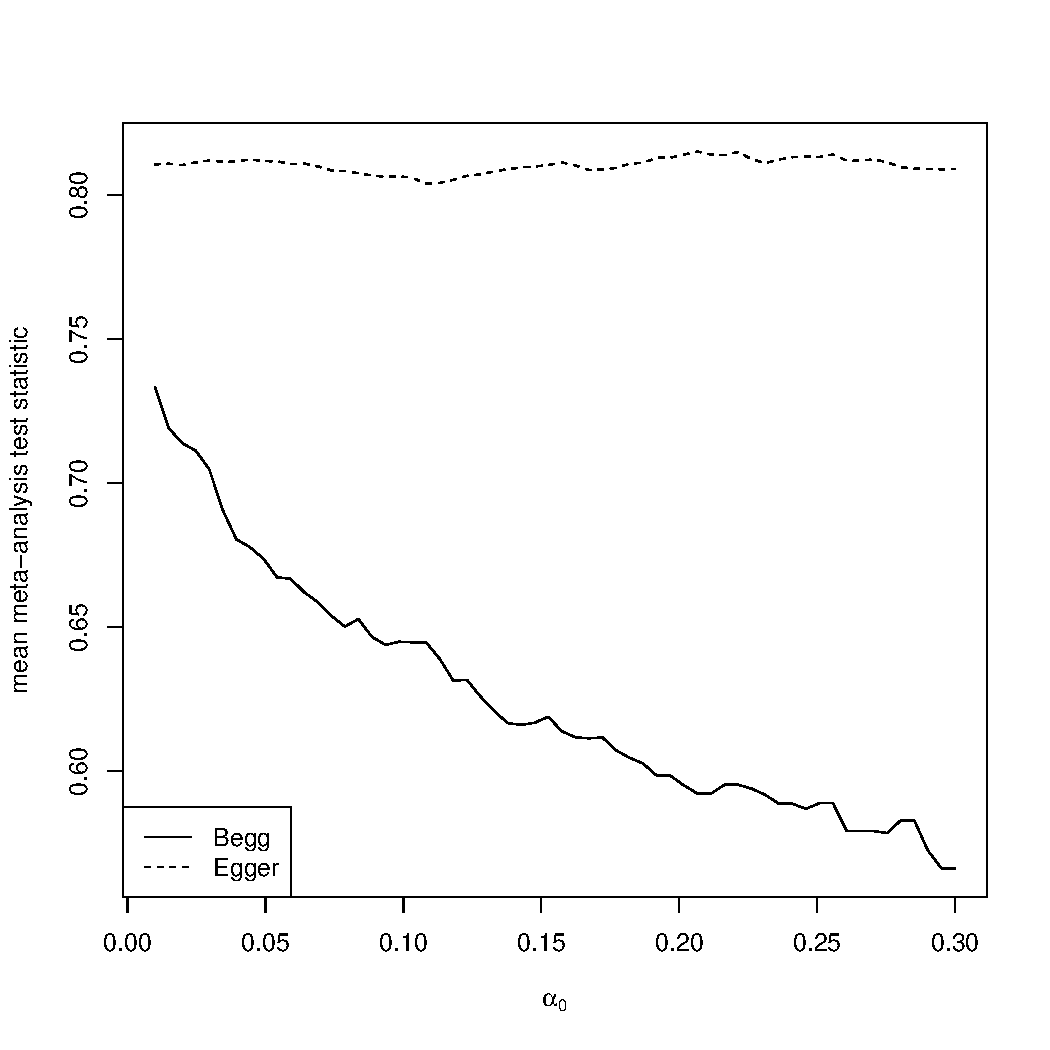
\includegraphics[width=\linewidth]{fig_alpha_0_beta.pdf}
%     \caption{Beta $f_\z$.}
%   \end{minipage}
% \end{figure}

\begin{figure}
\label{fig:alpha_0}
  \begin{subfigure}{.5\textwidth}
    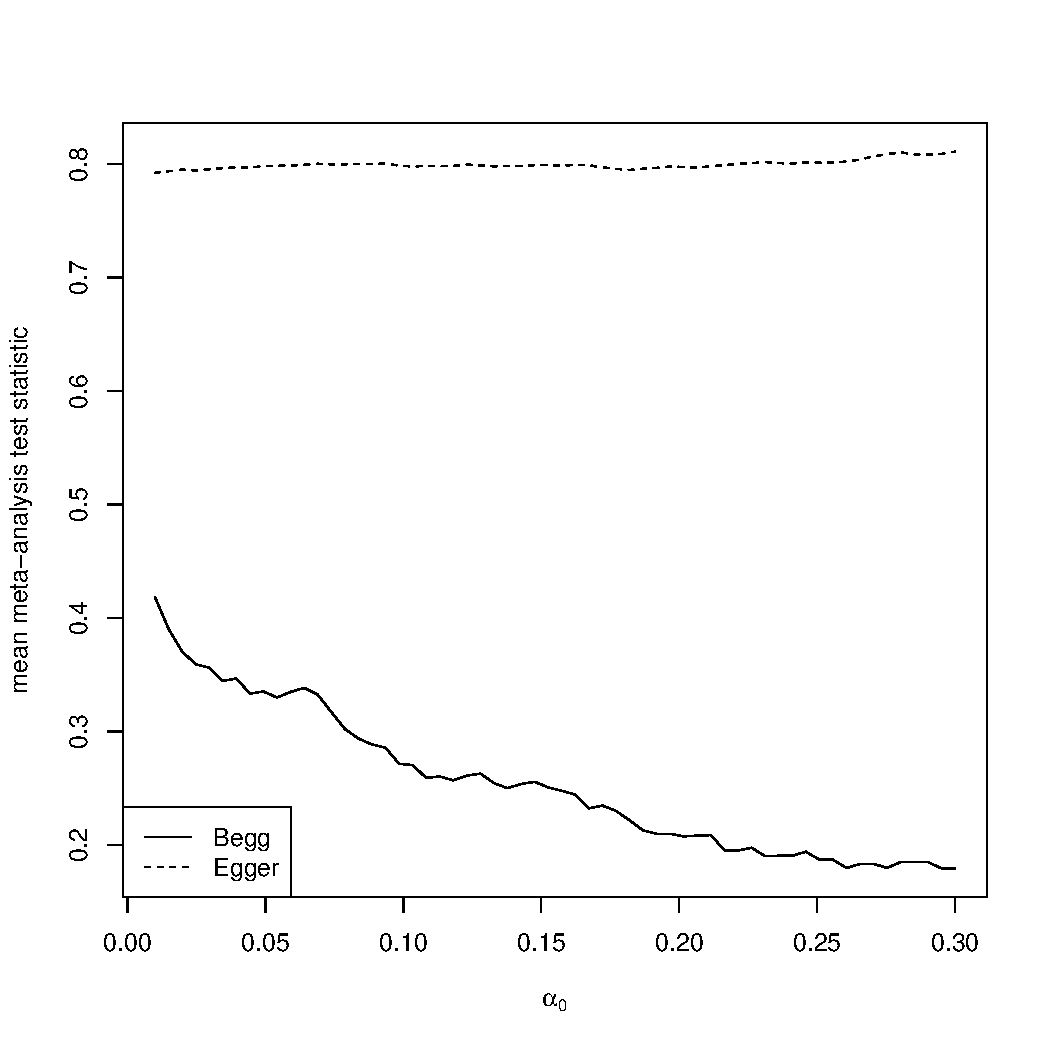
\includegraphics[width=\linewidth]{fig_alpha_0_power.pdf}
    \caption{Power-type $f_\z$.}
  \end{subfigure}
  \begin{subfigure}{.5\textwidth}
    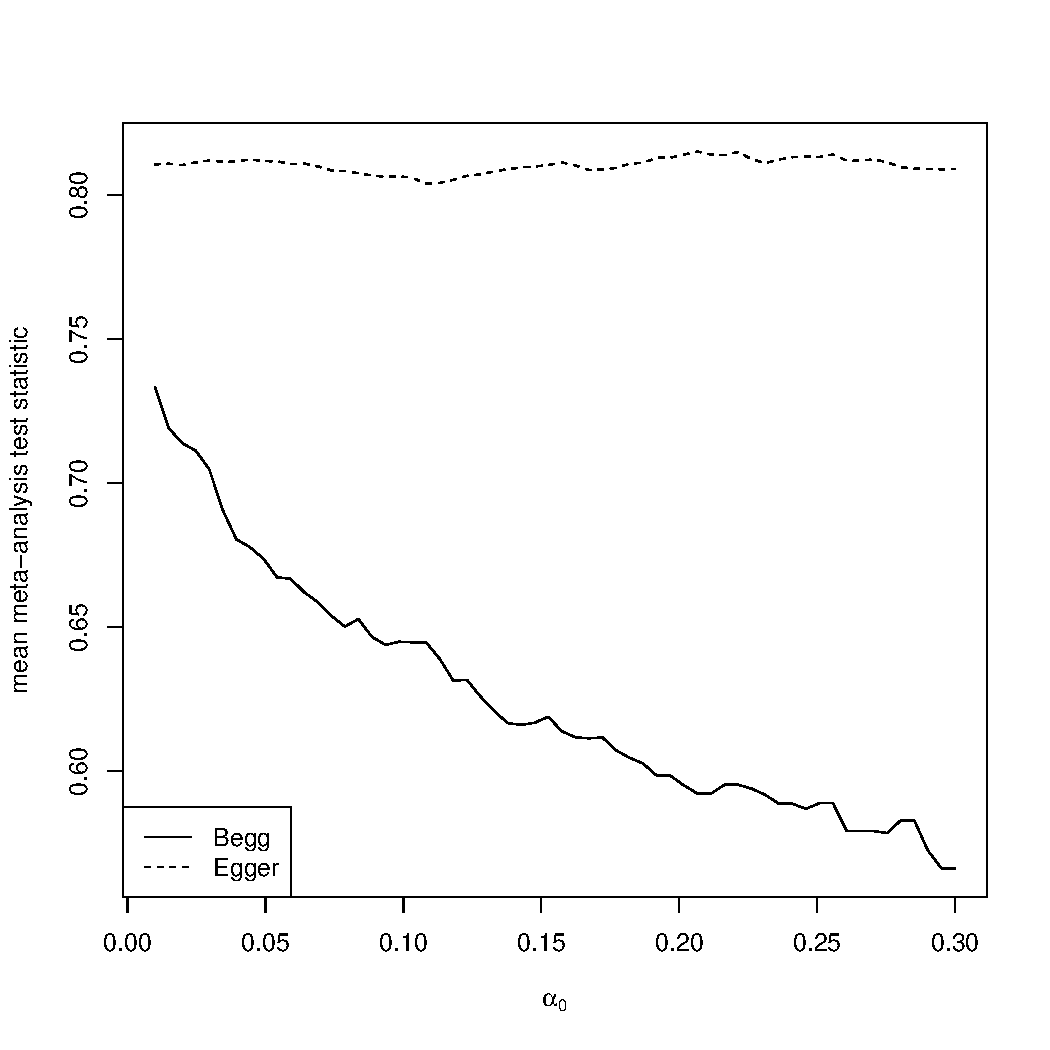
\includegraphics[width=\linewidth]{fig_alpha_0_beta.pdf}
    \caption{Beta $f_\z$.}
  \end{subfigure}
\caption{The effect of the nominal level $\alpha_0$ of the publication bias screen on the monte carlo mean of the meta-analysis test statistic.}\label{fig:alpha_0}
\end{figure}


Both of these ``counterintuitive results'' emerge in the simulation
analysis conducted by \citet{schucany:06} in their investigation of the effect of screening for
normality with the Shapiro-Wilks test.%, though it is not clear whether the underlying mechanisms are connected.
%
%\begin{table}
%% latex table generated in R 4.0.2 by xtable 1.8-4 package
% Mon Sep  5 15:46:04 2022
\begin{tabular}{lll |rrrrrrrrr}
  \hline
               &             & $f_Z$               & \multicolumn{1}{l}{     t} & \multicolumn{1}{l}{      } & \multicolumn{1}{l}{      } & \multicolumn{1}{l}{ power} & \multicolumn{1}{l}{      } & \multicolumn{1}{l}{      } & \multicolumn{1}{l}{  beta} & \multicolumn{1}{l}{      } & \multicolumn{1}{l}{      } \\ 
  condition     & $\alpha_0$ & n $\vert$ $\zeta$ & \multicolumn{1}{l}{   low} & \multicolumn{1}{l}{   med} & \multicolumn{1}{l}{  high} & \multicolumn{1}{l}{   low} & \multicolumn{1}{l}{   med} & \multicolumn{1}{l}{  high} & \multicolumn{1}{l}{   low} & \multicolumn{1}{l}{   med} & \multicolumn{1}{l}{  high} \\ 
   \hline
begg          & 0.05        & 25                  & 0.050 & 0.046 & 0.009 & 0.050 & 0.050 & 0.045 & 0.049 & 0.049 & 0.031 \\ 
                &             & 75                  & 0.050 & 0.047 & 0.008 & 0.051 & 0.049 & 0.007 & 0.050 & 0.049 & 0.020 \\ 
                & 0.15        & 25                  & 0.051 & 0.046 & 0.007 & 0.049 & 0.050 & 0.040 & 0.049 & 0.048 & 0.026 \\ 
                &             & 75                  & 0.050 & 0.047 & 0.006 & 0.050 & 0.048 & 0.005 & 0.051 & 0.048 & 0.015 \\ 
  egger         & 0.05        & 25                  & 0.050 & 0.048 & 0.012 & 0.050 & 0.050 & 0.052 & 0.049 & 0.049 & 0.049 \\ 
                &             & 75                  & 0.051 & 0.048 & 0.012 & 0.050 & 0.049 & 0.051 & 0.050 & 0.050 & 0.049 \\ 
                & 0.15        & 25                  & 0.051 & 0.048 & 0.012 & 0.049 & 0.050 & 0.053 & 0.049 & 0.049 & 0.048 \\ 
                &             & 75                  & 0.051 & 0.048 & 0.012 & 0.051 & 0.049 & 0.052 & 0.051 & 0.050 & 0.049 \\ 
  unconditional & 0.05        & 25                  & 0.050 & 0.047 & 0.012 & 0.050 & 0.050 & 0.052 & 0.049 & 0.050 & 0.049 \\ 
                &             & 75                  & 0.050 & 0.048 & 0.012 & 0.051 & 0.049 & 0.051 & 0.050 & 0.049 & 0.049 \\ 
                & 0.15        & 25                  & 0.050 & 0.047 & 0.012 & 0.050 & 0.050 & 0.052 & 0.049 & 0.050 & 0.049 \\ 
                &             & 75                  & 0.050 & 0.048 & 0.012 & 0.051 & 0.049 & 0.051 & 0.050 & 0.049 & 0.049 \\ 
   \hline
\end{tabular}

%\caption{$\theta=0$. }
%\end{table}
%\begin{table}
%% latex table generated in R 4.0.2 by xtable 1.8-4 package
% Mon Sep  5 15:46:04 2022
\begin{tabular}{lll |rrrrrrrrr}
  \hline
               &             & $f_Z$               & \multicolumn{1}{l}{     t} & \multicolumn{1}{l}{      } & \multicolumn{1}{l}{      } & \multicolumn{1}{l}{ power} & \multicolumn{1}{l}{      } & \multicolumn{1}{l}{      } & \multicolumn{1}{l}{  beta} & \multicolumn{1}{l}{      } & \multicolumn{1}{l}{      } \\ 
  condition     & $\alpha_0$ & n $\vert$ $\zeta$ & \multicolumn{1}{l}{   low} & \multicolumn{1}{l}{   med} & \multicolumn{1}{l}{  high} & \multicolumn{1}{l}{   low} & \multicolumn{1}{l}{   med} & \multicolumn{1}{l}{  high} & \multicolumn{1}{l}{   low} & \multicolumn{1}{l}{   med} & \multicolumn{1}{l}{  high} \\ 
   \hline
begg          & 0.05        & 25                  & 0.158 & 0.148 & 0.032 & 0.167 & 0.165 & 0.113 & 0.166 & 0.165 & 0.132 \\ 
                &             & 75                  & 0.393 & 0.389 & 0.279 & 0.396 & 0.394 & 0.049 & 0.395 & 0.393 & 0.272 \\ 
                & 0.15        & 25                  & 0.158 & 0.147 & 0.029 & 0.167 & 0.165 & 0.095 & 0.166 & 0.163 & 0.117 \\ 
                &             & 75                  & 0.393 & 0.386 & 0.266 & 0.396 & 0.392 & 0.025 & 0.396 & 0.390 & 0.235 \\ 
  egger         & 0.05        & 25                  & 0.159 & 0.150 & 0.039 & 0.167 & 0.167 & 0.160 & 0.166 & 0.167 & 0.170 \\ 
                &             & 75                  & 0.395 & 0.392 & 0.306 & 0.395 & 0.397 & 0.398 & 0.396 & 0.397 & 0.398 \\ 
                & 0.15        & 25                  & 0.159 & 0.151 & 0.040 & 0.168 & 0.166 & 0.162 & 0.166 & 0.167 & 0.168 \\ 
                &             & 75                  & 0.395 & 0.394 & 0.307 & 0.396 & 0.398 & 0.398 & 0.397 & 0.397 & 0.398 \\ 
  unconditional & 0.05        & 25                  & 0.159 & 0.149 & 0.037 & 0.168 & 0.166 & 0.158 & 0.167 & 0.167 & 0.169 \\ 
                &             & 75                  & 0.394 & 0.393 & 0.303 & 0.395 & 0.397 & 0.398 & 0.395 & 0.397 & 0.398 \\ 
                & 0.15        & 25                  & 0.159 & 0.149 & 0.037 & 0.168 & 0.166 & 0.158 & 0.167 & 0.167 & 0.169 \\ 
                &             & 75                  & 0.394 & 0.393 & 0.303 & 0.395 & 0.397 & 0.398 & 0.395 & 0.397 & 0.398 \\ 
   \hline
\end{tabular}

%\caption{$\theta=0.2.$}\label{table:power 0.2}
%\end{table}
%

\begin{figure}
 \begin{subfigure}{.5\textwidth}
    % latex table generated in R 4.0.2 by xtable 1.8-4 package
% Mon Sep  5 15:46:04 2022
\begin{tabular}{lll |rrrrrrrrr}
  \hline
               &             & $f_Z$               & \multicolumn{1}{l}{     t} & \multicolumn{1}{l}{      } & \multicolumn{1}{l}{      } & \multicolumn{1}{l}{ power} & \multicolumn{1}{l}{      } & \multicolumn{1}{l}{      } & \multicolumn{1}{l}{  beta} & \multicolumn{1}{l}{      } & \multicolumn{1}{l}{      } \\ 
  condition     & $\alpha_0$ & n $\vert$ $\zeta$ & \multicolumn{1}{l}{   low} & \multicolumn{1}{l}{   med} & \multicolumn{1}{l}{  high} & \multicolumn{1}{l}{   low} & \multicolumn{1}{l}{   med} & \multicolumn{1}{l}{  high} & \multicolumn{1}{l}{   low} & \multicolumn{1}{l}{   med} & \multicolumn{1}{l}{  high} \\ 
   \hline
begg          & 0.05        & 25                  & 0.050 & 0.046 & 0.009 & 0.050 & 0.050 & 0.045 & 0.049 & 0.049 & 0.031 \\ 
                &             & 75                  & 0.050 & 0.047 & 0.008 & 0.051 & 0.049 & 0.007 & 0.050 & 0.049 & 0.020 \\ 
                & 0.15        & 25                  & 0.051 & 0.046 & 0.007 & 0.049 & 0.050 & 0.040 & 0.049 & 0.048 & 0.026 \\ 
                &             & 75                  & 0.050 & 0.047 & 0.006 & 0.050 & 0.048 & 0.005 & 0.051 & 0.048 & 0.015 \\ 
  egger         & 0.05        & 25                  & 0.050 & 0.048 & 0.012 & 0.050 & 0.050 & 0.052 & 0.049 & 0.049 & 0.049 \\ 
                &             & 75                  & 0.051 & 0.048 & 0.012 & 0.050 & 0.049 & 0.051 & 0.050 & 0.050 & 0.049 \\ 
                & 0.15        & 25                  & 0.051 & 0.048 & 0.012 & 0.049 & 0.050 & 0.053 & 0.049 & 0.049 & 0.048 \\ 
                &             & 75                  & 0.051 & 0.048 & 0.012 & 0.051 & 0.049 & 0.052 & 0.051 & 0.050 & 0.049 \\ 
  unconditional & 0.05        & 25                  & 0.050 & 0.047 & 0.012 & 0.050 & 0.050 & 0.052 & 0.049 & 0.050 & 0.049 \\ 
                &             & 75                  & 0.050 & 0.048 & 0.012 & 0.051 & 0.049 & 0.051 & 0.050 & 0.049 & 0.049 \\ 
                & 0.15        & 25                  & 0.050 & 0.047 & 0.012 & 0.050 & 0.050 & 0.052 & 0.049 & 0.050 & 0.049 \\ 
                &             & 75                  & 0.050 & 0.048 & 0.012 & 0.051 & 0.049 & 0.051 & 0.050 & 0.049 & 0.049 \\ 
   \hline
\end{tabular}

    \caption{$\theta=0$}
\label{table:power 0}
  \end{subfigure}\\
  \begin{subfigure}{.5\textwidth}
	% latex table generated in R 4.0.2 by xtable 1.8-4 package
% Mon Sep  5 15:46:04 2022
\begin{tabular}{lll |rrrrrrrrr}
  \hline
               &             & $f_Z$               & \multicolumn{1}{l}{     t} & \multicolumn{1}{l}{      } & \multicolumn{1}{l}{      } & \multicolumn{1}{l}{ power} & \multicolumn{1}{l}{      } & \multicolumn{1}{l}{      } & \multicolumn{1}{l}{  beta} & \multicolumn{1}{l}{      } & \multicolumn{1}{l}{      } \\ 
  condition     & $\alpha_0$ & n $\vert$ $\zeta$ & \multicolumn{1}{l}{   low} & \multicolumn{1}{l}{   med} & \multicolumn{1}{l}{  high} & \multicolumn{1}{l}{   low} & \multicolumn{1}{l}{   med} & \multicolumn{1}{l}{  high} & \multicolumn{1}{l}{   low} & \multicolumn{1}{l}{   med} & \multicolumn{1}{l}{  high} \\ 
   \hline
begg          & 0.05        & 25                  & 0.158 & 0.148 & 0.032 & 0.167 & 0.165 & 0.113 & 0.166 & 0.165 & 0.132 \\ 
                &             & 75                  & 0.393 & 0.389 & 0.279 & 0.396 & 0.394 & 0.049 & 0.395 & 0.393 & 0.272 \\ 
                & 0.15        & 25                  & 0.158 & 0.147 & 0.029 & 0.167 & 0.165 & 0.095 & 0.166 & 0.163 & 0.117 \\ 
                &             & 75                  & 0.393 & 0.386 & 0.266 & 0.396 & 0.392 & 0.025 & 0.396 & 0.390 & 0.235 \\ 
  egger         & 0.05        & 25                  & 0.159 & 0.150 & 0.039 & 0.167 & 0.167 & 0.160 & 0.166 & 0.167 & 0.170 \\ 
                &             & 75                  & 0.395 & 0.392 & 0.306 & 0.395 & 0.397 & 0.398 & 0.396 & 0.397 & 0.398 \\ 
                & 0.15        & 25                  & 0.159 & 0.151 & 0.040 & 0.168 & 0.166 & 0.162 & 0.166 & 0.167 & 0.168 \\ 
                &             & 75                  & 0.395 & 0.394 & 0.307 & 0.396 & 0.398 & 0.398 & 0.397 & 0.397 & 0.398 \\ 
  unconditional & 0.05        & 25                  & 0.159 & 0.149 & 0.037 & 0.168 & 0.166 & 0.158 & 0.167 & 0.167 & 0.169 \\ 
                &             & 75                  & 0.394 & 0.393 & 0.303 & 0.395 & 0.397 & 0.398 & 0.395 & 0.397 & 0.398 \\ 
                & 0.15        & 25                  & 0.159 & 0.149 & 0.037 & 0.168 & 0.166 & 0.158 & 0.167 & 0.167 & 0.169 \\ 
                &             & 75                  & 0.394 & 0.393 & 0.303 & 0.395 & 0.397 & 0.398 & 0.395 & 0.397 & 0.398 \\ 
   \hline
\end{tabular}

    \caption{$\theta=0.2$}
		\label{table:power 0.2}
  \end{subfigure}
\caption{The observed false positive rate (\ref{table:power 0}) and power (\ref{table:power 0.2}) for meta-analyses conducted subsequent to a null finding on Egger's test or Begg's test and, for a benchmark, without any preliminary test. Three families were considered for the distribution $f_Z$ of the study effects, versions of Student's t, the power-law distribution, and beta distribution.  From each family, three distributions were used corresponding to a low, medium, or high value of $\zdiff$. For Student's t, the corresponding degrees of freedom were, respectively, 4, 3, and 2.1. For the power-law family \eqref{defn:peaked pdf}, the parameter was -.1, -.5, or -.9. For the beta family \eqref{defn:centered beta}, the common shape parameter was .9, .5, or .1.}\label{fig:table:power}
\end{figure}


% theorem [[ref]] is
%   asymptotic, and the convergence is slow as $p$ goes down to
%   $-.5$. the finite sample effect is less severe. more refined
%   asymptotic analysis needed.

% schucany and ng in simulations find both effects when screening for
% normality with shapiro-wilks. 1. the ``counterintuitive result'' that
% a smaller alpha at the screening stage is to be recommended.
% 2. ``Somewhat surprisingly, when the sample size increases, the
% conditional Type-I error rates increase, getting further away from the
% nominal rate'' theoretical justification given here, at least for pb
% screening.

\section {Conclusion}
\label{sec:conclusion}

The recommendation to test for publication bias before conducting a
meta-analysis is tentatively supported by many of the results presented here. The
exceptions involve screening on Begg's test with nonnormal data, in
which case the main effect is a loss of power of the meta-analysis,
arguably of less concern than a loss of FPR control. These conclusions
of course presuppose validity of the test assumptions, such as the
idealized fixed-effects model.

When screening by Begg's test does reduce the power of the subsequent
meta-analysis, it appears that larger sample sizes and using a larger
nominal level in the publication bias test both aggravate the issue.
That the power decreases with sample size is an artifact of our
asymptotic theory, which predicts a more severe dependency than
exhibited in finite samples. It is possible that with other
data-generating mechanisms the reverse trend occurs.

A lower nominal level is generally cautioned against as the two-stage
testing procedure involves accepting a narrow null hypothesis and
power is desirable. One possible remedy to choosing the appropriate
level is to use the asymptotic conditional distribution of the
meta-analysis statistic implied by Theorem \ref{thrm:begg asy}.

We give three avenues for further work. The foregoing analysis,
relying on the fixed-effects model, ignores the effect of
heterogeneity in screening. Second, the analysis only looks at the
effect of screening on true nulls. The effect of screening when
publication bias is present but the generally under-powered
publication bias test fails to identify is the complementary
analysis. This analysis requires a choice of model for publication
bias. Finally, another possible source of post-selection inference in
conducting meta-analysis is the test for heterogeneity. The effect of
choosing which type of meta-analysis to conduct based on the outcome
of the preliminary heterogeneity test may influence the main analysis.


\bibliographystyle{chicago}
\bibliography{screening.bib}

\end{document}

TODO

cosh optimization

use joint distribution of tauhat and thetahat to make simultaneous inference

after writing up proof linear expansion of begg statistic, add any
assumptions here

currently citing van der vaart, rao, and dembo's notes.